% Options for packages loaded elsewhere
\PassOptionsToPackage{unicode}{hyperref}
\PassOptionsToPackage{hyphens}{url}
\PassOptionsToPackage{dvipsnames,svgnames,x11names}{xcolor}
\documentclass[
  10pt,
  twocolumn]{article}
\usepackage{xcolor}
\usepackage[margin=0.75in]{geometry}
\usepackage{amsmath,amssymb}
\setcounter{secnumdepth}{5}
\usepackage{iftex}
\ifPDFTeX
  \usepackage[T1]{fontenc}
  \usepackage[utf8]{inputenc}
  \usepackage{textcomp} % provide euro and other symbols
\else % if luatex or xetex
  \usepackage{unicode-math} % this also loads fontspec
  \defaultfontfeatures{Scale=MatchLowercase}
  \defaultfontfeatures[\rmfamily]{Ligatures=TeX,Scale=1}
\fi
\usepackage{lmodern}
\ifPDFTeX\else
  % xetex/luatex font selection
\fi
% Use upquote if available, for straight quotes in verbatim environments
\IfFileExists{upquote.sty}{\usepackage{upquote}}{}
\IfFileExists{microtype.sty}{% use microtype if available
  \usepackage[]{microtype}
  \UseMicrotypeSet[protrusion]{basicmath} % disable protrusion for tt fonts
}{}
\makeatletter
\@ifundefined{KOMAClassName}{% if non-KOMA class
  \IfFileExists{parskip.sty}{%
    \usepackage{parskip}
  }{% else
    \setlength{\parindent}{0pt}
    \setlength{\parskip}{6pt plus 2pt minus 1pt}}
}{% if KOMA class
  \KOMAoptions{parskip=half}}
\makeatother
\usepackage{longtable,booktabs,array}
\usepackage{caption}
\captionsetup[table]{skip=6pt}
\newcounter{none} % for unnumbered tables
\usepackage{calc} % for calculating minipage widths
% Correct order of tables after \paragraph or \subparagraph
\usepackage{etoolbox}
\makeatletter
\patchcmd\longtable{\par}{\if@noskipsec\mbox{}\fi\par}{}{}
\makeatother
% Allow footnotes in longtable head/foot
\IfFileExists{footnotehyper.sty}{\usepackage{footnotehyper}}{\usepackage{footnote}}
\makesavenoteenv{longtable}
\usepackage{graphicx}
\makeatletter
\newsavebox\pandoc@box
\newcommand*\pandocbounded[1]{% scales image to fit in text height/width
  \sbox\pandoc@box{#1}%
  \Gscale@div\@tempa{\textheight}{\dimexpr\ht\pandoc@box+\dp\pandoc@box\relax}%
  \Gscale@div\@tempb{\linewidth}{\wd\pandoc@box}%
  \ifdim\@tempb\p@<\@tempa\p@\let\@tempa\@tempb\fi% select the smaller of both
  \ifdim\@tempa\p@<\p@\scalebox{\@tempa}{\usebox\pandoc@box}%
  \else\usebox{\pandoc@box}%
  \fi%
}
% Set default figure placement to htbp
\def\fps@figure{htbp}
\makeatother
\setlength{\emergencystretch}{3em} % prevent overfull lines
\providecommand{\tightlist}{%
  \setlength{\itemsep}{0pt}\setlength{\parskip}{0pt}}
\usepackage{bookmark}
\IfFileExists{xurl.sty}{\usepackage{xurl}}{} % add URL line breaks if available
\urlstyle{same}
% fallback for those not using the hyperref driver hyperxmp:
\makeatletter
\@ifundefined{xmpquote}{\newcommand{\xmpquote}[1]{#1}}{}
\makeatother
\hypersetup{
  colorlinks=true,
  linkcolor={blue},
  filecolor={Maroon},
  citecolor={Blue},
  urlcolor={Blue},
  pdfcreator={LaTeX via pandoc}}

\author{}
\date{}

\begin{document}

\section{Compositional Operators and Novelty Saturation in a Constrained
Procedural Spell
Grammar}\label{compositional-operators-and-novelty-saturation-in-a-constrained-procedural-spell-grammar}

\emph{A study of the Spellbox generation system}

\subsection{Abstract}\label{abstract}

Procedural content generators built on a small set of primitives often
face a tradeoff between structural validity and the richness of the
space they can produce. This paper studies that tradeoff in Spellbox, a
compositional spell-construction system built from a limited set of
primitive signs and two composition operators, nesting and linking. We
ask: \emph{how do compositional operators affect novelty saturation in a
constrained procedural generation grammar?} We test two hypotheses: (H1)
compositional operators significantly delay novelty saturation relative
to a flat (non-compositional) grammar, and (H2) increasing compositional
depth increases complexity at the cost of reduced structural validity.
Across six experiment families (varying generation volume, varying
maximum nesting depth, varying maximum linking depth, a repeated-reroll
discovery-rate study, and two generality checks: a constraint-aware
generator variant and a fully independent second grammar), run across 5
seeds where applicable and reported as mean ± standard deviation, we
find clear support for both hypotheses. A flat grammar (depth 0)
saturates quickly, with discovery rate falling from 79.4\% ± 1.9 to
12.4\% ± 0.8 over 30 re-rolls, while every nested or linked shape
sustains 76-96\% discovery rate across the same span: an absolute gap of
64-83 percentage points that only widens with depth. During this study
we discovered and corrected a methodological bug in which
uniqueness-ratio and discovery-rate tracking counted a
spell\textquotesingle s structural signature as "unique" or "newly
discovered" without gating on whether that spell was actually valid; a
parallel, validity-gated version of each metric was added alongside the
original (Section 2.2), and both are reported throughout. Under the
validity-gated metric, the flat baseline\textquotesingle s run-30
discovery rate is 11.1\% and compositional shapes sustain 70.6-89.2\%,
an absolute gap of roughly 60-78 percentage points, slightly smaller
than the original 64-83 point figure but not materially different: H1
and H2 verdicts are unchanged under the correction. At the same time,
raising nesting or linking depth from 0 to 30 drives structural validity
down from 87.9\% ± 0.4 to 25-26\% (a 70\% relative drop) while raw
complexity score rises 22-28×. We find H1 replicates in an independent
second grammar built for this study; H2 replicates cleanly for that
grammar\textquotesingle s nesting-equivalent operator but not for its
linking-equivalent operator, a genuine and reported divergence from
Spellbox. A constraint-aware generator variant recovers 6-19 percentage
points of validity at matched depth without moving discovery rate,
pinpointing composition-symbol incompatibility (not compositional depth
itself) as the dominant validity-loss mechanism. Per-seed model
selection (AIC/BIC) favors a logarithmic decay model for
discovery-rate-vs-reroll in most shapes and seeds. Because each spell
independently draws its own nesting/linking depth up to a
run\textquotesingle s ceiling rather than every spell reaching it, a
nominal "depth" is a sampling ceiling, not a level every generated spell
attains; we quantify the resulting sampler bias directly (Section 3.10)
and find it accounts for an effective generative space many orders of
magnitude smaller than the nominal combinatorial space at depth. All
discovery-rate and search-space findings are scoped to the
\texttt{signature()} equivalence relation used throughout (Section 2.2),
which may be coarser or finer than a human\textquotesingle s sense of "a
new spell"; we have not independently validated this relation against
human judgment, and readers should treat "novelty" in this paper as
"novelty under \texttt{signature()}," not a directly validated proxy for
perceived novelty.

\subsection{1. Introduction}\label{1-introduction}

\subsubsection{1.1 Background}\label{11-background}

Spellbox is a lightweight sandbox for generating spells from a small set
of primitive components (Control, Manifestation, and Transformation
signs) combined under a fixed set of composition rules, motivated by
fictional magic systems that emphasize composition over an
ever-expanding vocabulary of effects (notably the sigil-composition
magic of \emph{Witch Hat Atelier} and the improvisational spellcraft of
\emph{Mushoku Tensei}). The underlying research goal of the broader
project is to determine how much expressive range a small primitive set
plus a composition rule set can produce, and whether that range is
effectively bounded by convergence as generation scales up (see
\href{../plan.md}{plan.md}).

Two structural operators exist for combining primitives beyond a flat,
single-level spell: \textbf{nesting}, where effects are composed inside
one another so that they compound, and \textbf{linking}, where multiple
casts are chained to run side-by-side. A spell is either nested or
linked, never both, and each generated spell is scored by a \textbf{Raw
Score} built from its structural ingredients (sign counts, reversed
signs, composition symbols, nesting depth, and link count), which is
then passed through one of three normalization functions (Sigmoid,
Exponential, Arctan) to produce a bounded \textbf{Complexity Score} and
an associated tier (Novice, Apprentice, Adept, Master).

\subsubsection{1.2 Related Work}\label{12-related-work}

This study sits at the intersection of three lines of work in procedural
content generation (PCG) research.

\textbf{Grammar-based / rule-based PCG.} Generating content from a small
vocabulary combined via explicit composition or production rules is a
long-standing PCG strategy. Shape grammars originate with Stiny and Gips
(1971), who formalized generative specification of visual/spatial
content via production rules; Prusinkiewicz and Lindenmayer (1990)
developed the parallel L-system tradition for generating branching
structure (most directly demonstrated on plant morphology, but
structurally a nesting/recursion grammar in the same sense used here).
Müller et al. (2006) applied a shape-grammar formalism (CGA) to
procedural building generation, and Dormans (2010) used graph grammars
to generate mission and space structure for action-adventure levels, the
closest structural analogue in the PCG literature to this
paper\textquotesingle s nesting and linking operators, since both are
graph-composition operators over a small primitive vocabulary rather
than a spatial or L-system grammar. Smith and Mateas contribute two
directly relevant threads: an answer-set-programming approach that
declares a design space and samples from it (2011), directly relevant to
this paper\textquotesingle s Section 3.10 space-size analysis, and a
sculptable design-space approach to generating rulesets for mini-games
(2010). Shaker, Togelius, and Nelson\textquotesingle s textbook (2016)
surveys this area broadly and is cited here for the general
grammar-based PCG framing. Spellbox follows this tradition directly: a
fixed sign/sigil vocabulary plus two composition operators (nesting,
linking) define the entire generative grammar, and every generated spell
is a derivation of that grammar rather than free-form content.

\textbf{Expressive range and generator evaluation.} Smith and Whitehead
(2010) introduced expressive range analysis, characterizing a generator
by the distribution of outputs it produces along chosen metrics rather
than by inspecting individual outputs: the methodological ancestor of
this paper\textquotesingle s uniqueness-ratio and discovery-rate metrics
(Section 2.2). Summerville (2018) surveys and extends evaluation
methodologies for expressive range specifically. Cook et al. (2019)
introduce \emph{smoothness} and \emph{codependence} as general
analytical techniques for understanding how a
generator\textquotesingle s parameters map to its output space: the
single closest prior work to this paper\textquotesingle s depth sweeps
(Section 3.2), which are themselves an empirical smoothness/codependence
study of the nesting-depth and linking-depth parameters against
validity, complexity, and discovery rate. Cook et al. (2022) build
interactive tooling (Danesh) for this kind of generator analysis. Horn
et al. (2014) provide a comparative empirical evaluation of several
procedural level generators sharing a common test framework,
methodologically similar in spirit to this paper\textquotesingle s
second-grammar generality check (Section 3.7). Smith (2017) frames the
broader question of what PCG research should value, directly relevant to
this paper\textquotesingle s discussion of the validity-versus-novelty
tradeoff (Section 4.1).

\textbf{Diversity and novelty in generated content.} Lehman and Stanley
(2011) introduce novelty as an explicit search objective distinct from
an extrinsic quality objective: the conceptual origin of treating
"novelty" as a first-class, measurable target, which this
paper\textquotesingle s H1 framing (novelty saturation as the primary
dependent variable) builds on directly. Mouret and Clune (2015) and the
quality-diversity framing of Pugh et al. (2016) and Gravina et al.
(2019) generalize this into an explicit quality-versus-diversity axis;
Gravina et al.\textquotesingle s framing in particular is close to a
relabeling of this paper\textquotesingle s validity-versus-novelty
tradeoff (H1 vs. H2) in different terminology. This
paper\textquotesingle s discovery-rate methodology and Section
3.10\textquotesingle s per-depth uniqueness reachability are
conceptually adjacent to a MAP-Elites-style archive (Mouret and Clune
2015) restricted to a single "how novel" axis rather than a full
behavioral map. Togelius et al. (2011) survey search-based PCG broadly,
including the exploration-exploitation framing this
paper\textquotesingle s H1/H2 pair instantiates for a specific
two-operator grammar.

\textbf{Generative-space comparison.} For directly comparing
generators\textquotesingle{} reachable spaces (relevant to Section
3.7\textquotesingle s cross-grammar comparison and Section
3.8\textquotesingle s cross-generator comparison), Withington and
Tokarchuk propose methods for compressing and comparing PCG generative
spaces, and Barthet et al. propose a generative-shift analysis for
comparing generator behavior; both offer alternative, more formal
comparison methodologies than this paper\textquotesingle s depth-matched
metric tables, and are noted here as directions for a more rigorous
cross-generator comparison in future work.

This paper does not claim to introduce a new PCG technique; its
contribution is an empirical case study quantifying how two specific
composition operators trade off novelty retention against validity in a
constrained grammar, replicated in part against an independent second
grammar and an independent generator design change, both purpose-built
for this study (Sections 3.7-3.8), together with a general method
(Section 3.10) for quantifying how much of a compositional
grammar\textquotesingle s \emph{nominal} combinatorial space a given
sampling strategy actually reaches in practice.

\subsubsection{1.3 Research Question}\label{13-research-question}

\textbf{How do compositional operators affect novelty saturation in a
constrained procedural generation grammar?}

Novelty saturation, here, is operationalized as \textbf{discovery rate}:
across repeated re-rolls of the same generation shape (same amount, same
nesting-or-linking depth) with a new random seed each time, what
fraction of each roll\textquotesingle s output is structurally new
versus a repeat of something already seen? A grammar with a small
effective solution space saturates quickly: new rolls mostly reproduce
old spells. A grammar with a large effective solution space stays
"fresh" much longer.

\subsubsection{1.4 Hypotheses}\label{14-hypotheses}

\begin{itemize}
\tightlist
\item
  \textbf{H1 (Primary):} Compositional operators (nesting and linking)
  significantly delay novelty saturation compared with a flat grammar.
\item
  \textbf{H2 (Secondary):} Increasing compositional depth increases
  complexity at the cost of reduced validity.
\end{itemize}

\subsection{2. Methodology}\label{2-methodology}

\subsubsection{2.1 Generation Model}\label{21-generation-model}

All spells are produced by a bulk metrics generator parameterized by:
\textbf{amount} (spell count for the run), \textbf{max nesting depth},
\textbf{max linking depth}, a \textbf{normalization function}, and a
\textbf{seed}. Nesting and linking depth are mutually exclusive per run
in the sweep experiments (one is fixed at 0 while the other varies),
isolating each operator\textquotesingle s effect. Each generated spell
independently draws a nesting depth or link count between 0 and the
run\textquotesingle s ceiling, so the ceiling bounds the \emph{maximum}
achievable structural depth without forcing every spell to reach it.

\subsubsection{2.2 Metrics}\label{22-metrics}

\begin{itemize}
\tightlist
\item
  \textbf{Validity \%}: share of generated spells that are structurally
  sound (no broken composition rules); minor warnings do not count
  against this.
\item
  \textbf{Average Uniqueness Ratio}: fraction of spells in a single run
  that are structurally distinct from each other (within-run
  duplication).
\item
  \textbf{Average Raw Score / Average Complexity Score}: pre- and
  post-normalization complexity, averaged across a run.
\item
  \textbf{Modal Complexity Tier}: the tier occupied by the
  \emph{plurality} of spells in a run (a statistical mode, not the
  single most complex spell produced).
\item
  \textbf{Discovery Rate}: a cross-run metric distinct from uniqueness
  ratio. For a fixed generation shape re-rolled across a sequence of
  runs with ascending seeds, a persistent set of every distinct spell
  signature seen so far is maintained; each run\textquotesingle s
  discovery rate is \texttt{newCount\ /\ total} for that run alone. A
  flat, high discovery rate across many re-rolls indicates an
  unsaturated space; a falling rate indicates the space is being
  exhausted.
\end{itemize}

\textbf{A validity-gating bug, found and corrected.} During this study
we found that \texttt{signature()} was computed for every generated
spell regardless of structural validity, and every uniqueness-tracking
and discovery-tracking Set added that signature with no gate on
\texttt{record.valid}. Concretely, both the within-run uniqueness ratio
and the cross-run discovery rate treated an \emph{invalid}
spell\textquotesingle s signature exactly like a valid one: an invalid
spell could be counted as "unique" within a run, or as a "newly
discovered" signature across re-rolls, even though it was never a
structurally sound spell in the first place. This conflates two distinct
properties, "structurally distinct" and "structurally distinct and
valid", that the original metrics did not separate.

We fixed this by adding a parallel, validity-gated metric alongside each
existing (unfiltered) one, rather than replacing the original:

\begin{itemize}
\tightlist
\item
  \textbf{Uniqueness Ratio (valid-only)}:
  \texttt{uniquenessRatioValidOnly\ =\ uniqueValidSignatures\ /\ validCount},
  the fraction of a run\textquotesingle s \emph{valid} spells that are
  also structurally unique among the valid subset. The denominator is
  the count of valid spells, not the total spell count, so a shape with
  low overall validity is not double-penalized for a low validity rate
  it has already been charged for elsewhere.
\item
  \textbf{Discovery Rate (valid-only)}:
  \texttt{discoveryRatePctValidOnly\ =\ newValidCount\ /\ validTotal}
  per run, the fraction of a batch\textquotesingle s \emph{valid} spells
  that are newly-seen valid signatures, tracked against a persistent set
  of previously-seen valid signatures only.
\end{itemize}

Both the original and the validity-gated metric are reported side by
side everywhere in this paper that uniqueness ratio or discovery rate
appears (Sections 3.2, 3.3, 3.5, 3.7, 3.8, 3.10), so readers can judge
the size of the correction directly rather than take a single recomputed
number on faith. As Sections 3.2 and 3.3 report in detail, this
correction turns out to matter little for uniqueness ratio (at most
\textasciitilde1.2 points of difference) but matters more for discovery
rate at higher depth, where the gap between the two metrics reaches 6-7
points by run 30. Neither correction changes this
paper\textquotesingle s H1 or H2 verdicts (Section 3.6).

Full formal definitions are given in \url{compiled-analysis.md}, which
this paper treats as a canonical single-seed data source and leaves
unmodified.

\subsubsection{2.3 Experiment Design}\label{23-experiment-design}

Six experiment families were run in total:

\begin{enumerate}
\def\labelenumi{\arabic{enumi}.}
\tightlist
\item
  \textbf{Varying Amount of Spells} (single seed \texttt{12345}): amount
  swept from 12 to 120,000 at fixed shape (Max Nesting = 4, Max Linking
  = 0, and the mirror Max Nesting = 0, Max Linking = 4), plus a depth-0
  baseline, across all three normalization functions. Reported in full
  in \url{compiled-analysis.md}; summarized here in Section 3.1.
\item
  \textbf{Varying Max Nesting Depth, multi-seed}: depth swept over \{0,
  5, 10, 15, 20, 25, 30\} at fixed amount (1200), Max Linking = 0,
  Exponential normalization, across \textbf{5 independent seeds (1-5)},
  reported as mean ± standard deviation.
\item
  \textbf{Varying Max Linking Depth, multi-seed}: identical design to
  (2) with Max Nesting = 0, Max Linking swept, mirroring experiment 2 to
  allow direct nesting-vs-linking comparison.
\item
  \textbf{Discovery Rate, multi-seed}: 7 generation shapes (a depth-0
  baseline, three nesting depths, three linking depths, all at fixed
  amount = 1200) were each re-rolled 30 times in sequence, using
  Exponential normalization. This was repeated for \textbf{5 independent
  seed-anchors}, giving 5 independent 30-run trajectories per shape,
  reported as mean ± standard deviation at each run index.
\item
  \textbf{Second Grammar (Rune-Chain)}: a fully independent toy grammar
  with its own primitives, its own nesting-equivalent ("refinement") and
  linking-equivalent ("chaining") operators, its own validity rule, and
  its own scoring function was built and swept the same way (amount
  sweep, depth sweep, discovery-rate sequence, 5 seeds) to test whether
  H1/H2 generalize beyond Spellbox\textquotesingle s specific rule set.
\item
  \textbf{Constraint-Aware Generator Comparison}: the same depth sweeps
  and discovery-rate shapes as (2)-(4) were re-run under a second
  generator variant that biases the random sigil-pairing decision inside
  composition symbols toward known-compatible pairs, to isolate how much
  of the validity loss in (2)-(4) is attributable to that one decision
  point versus compositional depth itself.
\end{enumerate}

Multi-seed reruns (2-4) use seeds 1-5 directly for the depth sweeps, and
seed-anchors 1-5 (each expanded into a 30-run sequence via
\texttt{anchor\ ×\ 1000\ +\ runIndex}) for the discovery-rate sequences,
so no seed collides across sequences or with the single-seed
\texttt{12345} runs from experiment 1.

\subsection{3. Results}\label{3-results}

\subsubsection{3.1 Effect of Generation Volume
(Amount)}\label{31-effect-of-generation-volume-amount}

\emph{(Single seed \texttt{12345}; full table in
\url{compiled-analysis.md}.)}

Increasing the amount of spells generated per run improves validity but
degrades within-run uniqueness. Validity rises from 67\% to 77\% for
nested spells (Max Nesting = 4) and from 73\% to 88\% for linked spells
(Max Linking = 4) as amount increases from 12 to 120,000, plateauing
rather than climbing indefinitely. Uniqueness falls sharply over the
same range: from 1.00 to 0.69 for nested spells (a 31\% relative drop)
and much more severely from 1.00 to 0.12 for linked spells (an 88\%
relative drop); at the largest linked-spell run, only 12\% of generated
spells are structurally distinct from one another. Average raw score
stays roughly flat across the sweep, while average complexity score
under each normalization function tracks raw score\textquotesingle s
stability with fixed ordering \textbf{Sigmoid \textgreater{} Exponential
\textgreater{} Arctan}. Across all 30 tested amount/shape/normalization
combinations, linked spells never exceeded Novice tier, while nested
spells reached Apprentice or Adept; no combination reached Master.

\subsubsection{3.2 Effect of Compositional Depth (Multi-Seed, Mean ±
Std, n =
5)}\label{32-effect-of-compositional-depth-multi-seed-mean--std-n--5}

Nesting and linking depth were swept independently from 0 to 30 (fixed
amount = 1200, Exponential normalization) across 5 seeds. Both operators
show the same qualitative pattern (rising complexity, falling validity)
with low seed-to-seed variance throughout (validity std ≤ 2.6 points,
raw-score std ≤ 2.0 at every depth), confirming the single-seed trend
from the original sweep is not a seed-specific artifact:

\begin{table*}[t]
\centering
\begin{tabular}{@{}ccccc@{}}
\toprule
Depth & Nesting: Validity \% (mean ± std) & Nesting: Raw Score (mean ±
std) & Linking: Validity \% (mean ± std) & Linking: Raw Score (mean ±
std) \\
\midrule
0 & 87.9 ± 0.4 & 4.22 ± 0.04 & 87.9 ± 0.4 & 4.22 ± 0.04 \\
5 & 72.0 ± 1.1 & 18.04 ± 0.33 & 71.6 ± 1.2 & 14.75 ± 0.16 \\
10 & 56.0 ± 1.0 & 38.08 ± 0.55 & 57.5 ± 2.6 & 29.55 ± 0.66 \\
15 & 44.3 ± 0.6 & 58.77 ± 0.72 & 45.1 ± 0.6 & 45.53 ± 0.55 \\
20 & 36.1 ± 1.3 & 78.05 ± 0.76 & 36.2 ± 1.1 & 60.87 ± 1.26 \\
25 & 29.7 ± 1.2 & 99.81 ± 1.45 & 31.1 ± 1.8 & 76.66 ± 2.03 \\
30 & 25.7 ± 0.5 & 119.97 ± 1.31 & 25.1 ± 1.4 & 91.80 ± 1.94 \\
\bottomrule
\end{tabular}
\end{table*}

\textbf{Effect sizes:} from depth 0 to depth 30, validity drops from
87.9\% to 25-26\% for both operators: a \textbf{70.7\% relative decline}
for nesting and \textbf{71.4\%} for linking. Over the same range, raw
score rises from 4.22 to 119.97 for nesting (\textbf{28.4× increase})
and to 91.80 for linking (\textbf{21.8× increase}).
Nesting\textquotesingle s raw-score advantage over linking at matched
depth grows from negligible at depth 5 (18.04 vs. 14.75, +22\%) to
+30.7\% at depth 30 (119.97 vs. 91.80), while validity tracks within 1-2
points of each other at every depth, confirming this gap is a
scoring-weight artifact (nesting contributes 4 raw-score points per
level vs. 2 for linking beyond the first branch), not a difference in
how each operator affects structural soundness.

\textbf{Depth is a ceiling, not a level.} As noted in Section 2.1, each
spell independently draws its own nesting depth (or link count)
uniformly between 0 and the run\textquotesingle s ceiling, rather than
every spell in a "depth = 20" run actually reaching depth 20. We
instrumented the same draw used by the generator to report the
\emph{achieved} per-spell depth distribution at each configured ceiling:

\begin{table*}[t]
\centering
\begin{tabular}{@{}ccccccc@{}}
\toprule
Ceiling & Achieved nesting: mean & Achieved nesting: median & Achieved
nesting: range & Achieved linking: mean & Achieved linking: median &
Achieved linking: range \\
\midrule
5 & 2.45 & 2 & {[}0, 5{]} & 2.49 & 2 & {[}0, 5{]} \\
10 & 4.89 & 5 & {[}0, 10{]} & 4.98 & 5 & {[}0, 10{]} \\
15 & 7.39 & 7 & {[}0, 15{]} & 7.46 & 7 & {[}0, 15{]} \\
20 & 9.81 & 10 & {[}0, 20{]} & 9.96 & 10 & {[}0, 20{]} \\
25 & 12.28 & 12 & {[}0, 25{]} & 12.46 & 12 & {[}0, 25{]} \\
30 & 14.78 & 15 & {[}0, 30{]} & 14.95 & 15 & {[}0, 30{]} \\
\bottomrule
\end{tabular}
\end{table*}

At every ceiling, the achieved mean/median sits almost exactly at half
the ceiling (consistent with a uniform draw on
\texttt{{[}0,\ ceiling{]}}, whose expectation is
\texttt{ceiling\ /\ 2}), and the full range \texttt{{[}0,\ ceiling{]}}
is realized in every run. A "depth = 20" run\textquotesingle s 1200
spells therefore span the \emph{entire} range from depth-0 spells to
depth-20 spells, with a mean achieved depth of only 9.81, meaning every
row in the table above is already an average over a wide mixture of
shallow and deep spells, not a measurement of "spells at that depth."
This does not invalidate the depth-vs-validity/complexity trend (higher
ceilings do shift the whole achieved-depth distribution upward, and the
reported metrics move accordingly), but it means "the effect of depth"
in this section should be read as "the effect of raising the ceiling of
a per-spell uniform depth draw," not "the effect of forcing every spell
to a fixed depth." Section 3.10 shows this same mechanism (independent
per-spell depth draws concentrating mass at shallow depths) is also the
reason the observed vs. theoretical search-space gap widens so
dramatically with the ceiling.

\textbf{A geometric-decay baseline for H2.} If a spell is invalid
whenever any independently-checked node in its structure fails a
validity check, the simplest null model is that \texttt{P(valid)} decays
geometrically in the number of checked nodes:
\texttt{P(valid)\ ≈\ (1\ −\ p\_error)\^{}n}, where \texttt{p\_error} is
the per-node error probability and \texttt{n\ =\ depth\ +\ 1} is the
node count. \texttt{spellValidator.ts}\textquotesingle s error-level
checks are (a) a missing Control-category sign, and (b) an incompatible
Radial composition-symbol pair; inspecting
\texttt{spellBuilder.ts}\textquotesingle s \texttt{getSign()} shows
every one of its three sign-option branches always includes exactly one
Control-sign draw, so (a) never actually occurs in generator output; the
only real per-node error source is (b), driven by the 1-in-3 chance of
drawing a Radial composition symbol combined with the 9-in-25 chance
that pair includes at least one "Light" sigil
(\texttt{compatibility.ts}\textquotesingle s only incompatible
category). We measured this directly by generating 200,000 independent
depth-0 nodes and validating each one, giving an empirical
\texttt{p\_error\ =\ 0.1197}, closely matching the
\texttt{(1/3)(9/25)\ =\ 0.12} value predicted from the draw
probabilities directly. Comparing the resulting geometric-decay
prediction against the observed nesting-depth validity curve:

\begin{table*}[t]
\centering
\begin{tabular}{@{}ccccc@{}}
\toprule
Depth & Node count & Predicted \texttt{P(valid)} (geometric) & Observed
validity \% & Deviation \\
\midrule
0 & 1 & 88.0\% & 87.9\% & −0.1 pts \\
5 & 6 & 46.5\% & 72.0\% & +25.4 pts \\
10 & 11 & 24.6\% & 56.0\% & +31.4 pts \\
15 & 16 & 13.0\% & 44.3\% & +31.3 pts \\
20 & 21 & 6.9\% & 36.1\% & +29.2 pts \\
25 & 26 & 3.6\% & 29.7\% & +26.1 pts \\
30 & 31 & 1.9\% & 25.7\% & +23.8 pts \\
\bottomrule
\end{tabular}
\end{table*}

The geometric baseline matches the observed curve closely at depth 0 (as
it must, since a depth-0 spell has exactly one node and no compounding),
but \textbf{badly underpredicts} observed validity at every deeper
ceiling: by depth 10 the naive independent-conjunction model predicts
less than half the actually-observed validity, and the gap stays at
roughly +25-31 points across the rest of the range rather than closing.
This deviation is itself the interesting result, and it is explained by
the same mechanism as the paragraph above: node count
\texttt{n\ =\ depth\ +\ 1} assumes every spell in a "depth = d" run
actually has \texttt{d\ +\ 1} nodes, but the achieved-depth table shows
the \emph{true} mean node count at ceiling 20 is only
\texttt{9.81\ +\ 1\ ≈\ 10.8}, not \texttt{21}. Recomputing the geometric
prediction using the \emph{achieved} mean depth instead of the ceiling,
\texttt{(1\ −\ 0.1197)\^{}(9.81+1)\ =\ 30.4\%} at ceiling 20, closes
most of the gap (30.4\% vs. an observed 36.1\%, a residual of only +5.7
points, compared to +29.2 points using the ceiling). The remaining small
residual is consistent with the per-spell depth draw being a
\emph{distribution} rather than a point mass at the mean: geometric
decay is convex in \texttt{n}, so averaging \texttt{(1-p)\^{}n} over a
distribution of \texttt{n} values is always somewhat larger than
\texttt{(1-p)} raised to the \emph{mean} of that distribution
(Jensen\textquotesingle s inequality), which is exactly the direction
and rough scale of the residual observed here.
\textbf{H2\textquotesingle s validity-vs-depth curve is therefore almost
entirely explained by two facts that are not about compositional
structure being special: (1) a simple conjunction-of-independent-checks
model, and (2) the per-spell depth draw being a ceiling rather than a
level.} The genuinely interesting result in this paper\textquotesingle s
validity analysis is not that validity falls with depth (that is close
to a definitional consequence of the two facts above), but Section
3.8\textquotesingle s finding that a substantial share of the per-node
error rate itself (the \texttt{p\_error\ ≈\ 0.12} measured here) is
attributable to one fixable random-choice bottleneck, and is not an
intrinsic property of composition.

Uniqueness ratio \emph{rises} with depth for both operators, from 0.778
± 0.010 at depth 0 to 0.998 ± 0.002 (nesting) and 0.999 ± 0.001
(linking) at depth 30, the opposite direction from the amount
sweep\textquotesingle s uniqueness decay (Section 3.1). This is
expected: adding depth multiplies the number of structurally distinct
outcomes reachable per generation, so at fixed amount (1200), a larger
reachable space means fewer within-run collisions, even as
\emph{validity} among those same outputs collapses. Depth and amount
therefore pull uniqueness in opposite directions through two different
mechanisms: one shrinks the sample-to-space ratio (depth), the other
grows the sample at fixed space (amount).

\textbf{Valid-only recheck.} Applying the validity-gated uniqueness
metric (Section 2.2) to this same sweep (n = 5 seeds, amount = 1200)
gives:

\begin{table*}[t]
\centering
\begin{tabular}{@{}cccccc@{}}
\toprule
Depth & Validity \% & Nesting: Uniqueness (all) & Nesting: Uniqueness
(valid-only) & Linking: Uniqueness (all) & Linking: Uniqueness
(valid-only) \\
\midrule
0 & 87.9 & 0.7778 & 0.7659 & 0.7778 & 0.7659 \\
5 & 72.0 / 71.6 & 0.9582 & 0.9463 & 0.9687 & 0.9611 \\
10 & 56.0 / 57.5 & 0.9900 & 0.9833 & 0.9892 & 0.9828 \\
15 & 44.3 / 45.1 & 0.9960 & 0.9925 & 0.9948 & 0.9889 \\
20 & 36.1 / 36.2 & 0.9972 & 0.9920 & 0.9970 & 0.9922 \\
25 & 29.7 / 31.1 & 0.9983 & 0.9949 & 0.9977 & 0.9923 \\
30 & 25.7 / 25.1 & 0.9985 & 0.9941 & 0.9992 & 0.9968 \\
\bottomrule
\end{tabular}
\end{table*}

The corrected, validity-gated uniqueness ratio moves very little
relative to the original at every depth (at most \textasciitilde1.2
points, at depth 5), confirming this section\textquotesingle s claim
that "uniqueness rises with depth because the reachable space explodes"
is not materially distorted by the validity-gating bug described in
Section 2.2. This is one of the two cases in this paper (the other being
the ablation, Section 3.5) where the bug turns out not to change the
reported finding, and we say so plainly rather than implying a
correction was needed here when it was not.

\subsubsection{3.3 Discovery Rate Across Repeated Re-Rolls (Multi-Seed,
Mean ± Std, n =
5)}\label{33-discovery-rate-across-repeated-re-rolls-multi-seed-mean--std-n--5}

\pandocbounded{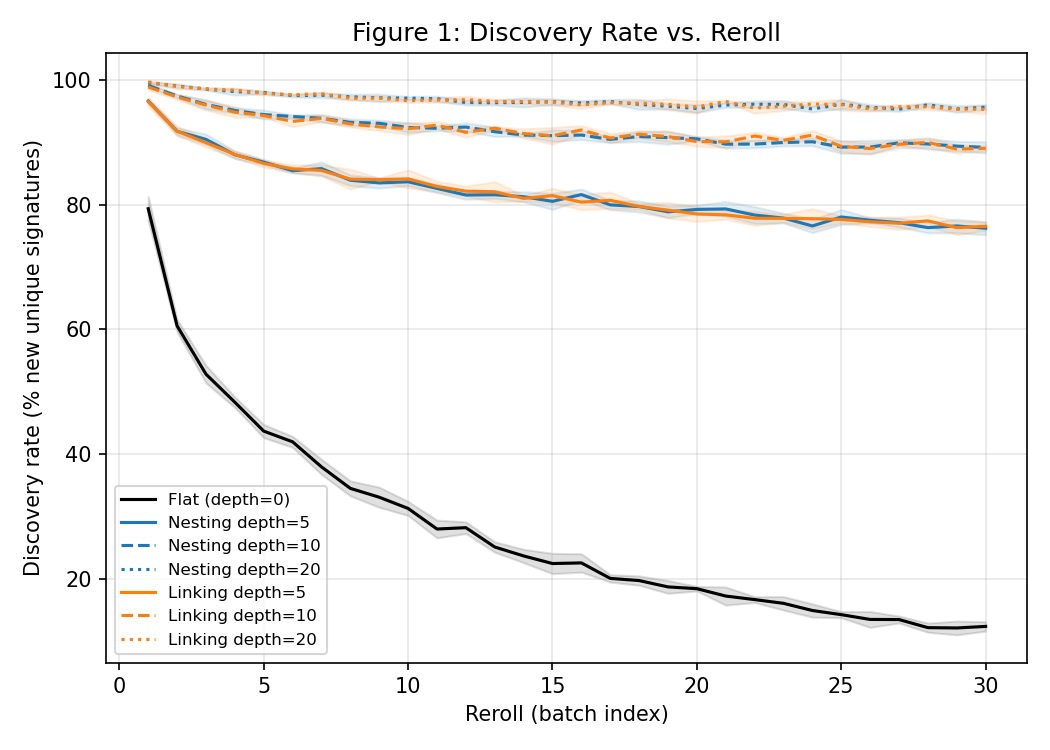
\includegraphics[keepaspectratio,alt={Figure 1: Discovery rate vs. reroll, flat vs. nesting vs. linking}]{figures/figure1_discovery_rate.png}}

\textbf{Figure 1.} Discovery rate (mean ± std band across 5
seed-anchors) vs. reroll index, for the flat baseline and three depths
each of nesting and linking. The flat shape (black) decays sharply and
continuously; every compositional shape (blue/orange) sustains a far
higher, more slowly-decaying discovery rate, with the gap widening as
depth increases.

\pandocbounded{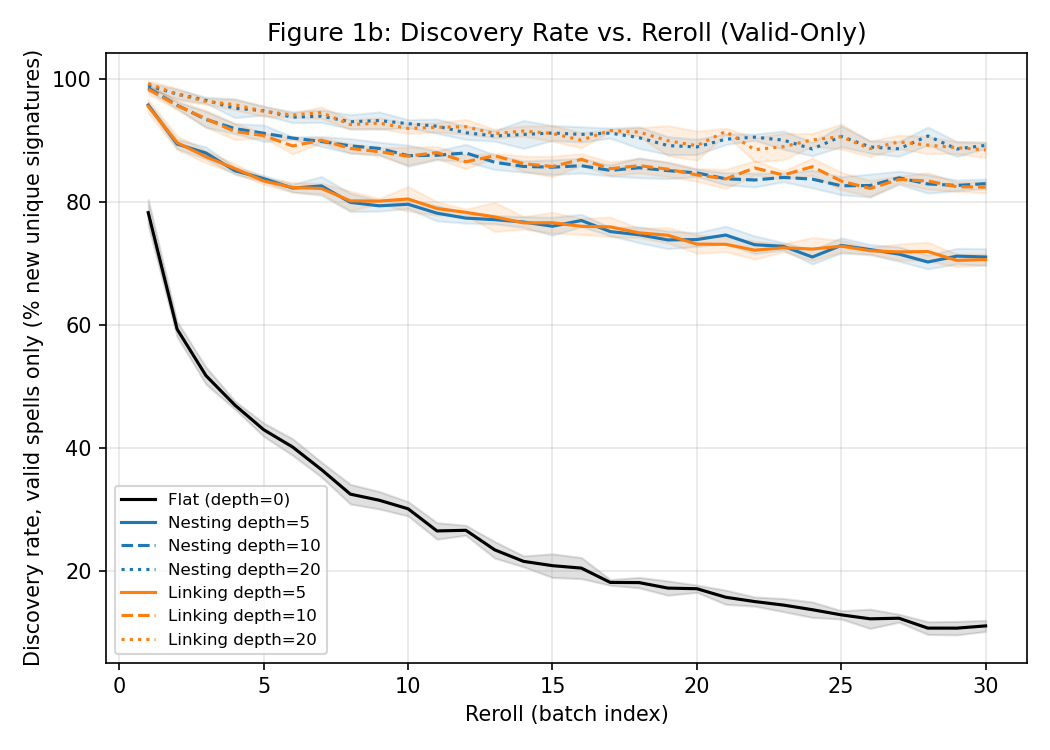
\includegraphics[keepaspectratio,alt={Figure 1b: Discovery rate vs. reroll, valid-only}]{figures/figure1b_discovery_rate_valid_only.png}}

\textbf{Figure 1b.} The same discovery-rate sequences as Figure 1,
recomputed under the validity-gated metric (Section 2.2). The overall
shape is unchanged: the flat baseline still collapses quickly and every
compositional shape still sustains a far higher rate, but each
compositional curve sits visibly lower than its Figure 1 counterpart,
most noticeably at higher depth, reflecting the 6-7 point gap quantified
in the tables below.

\begin{table*}[t]
\centering
\begin{tabular}{@{}lcccccc@{}}
\toprule
Shape & First-run discovery rate (all) & First-run (valid-only) & Run-30
discovery rate (all) & Run-30 (valid-only) & Absolute drop (all) &
Absolute drop (valid-only) \\
\midrule
Flat (depth 0) & 79.4\% ± 1.9 & 78.24\% ± 2.11 & 12.4\% ± 0.8 & 11.14\%
± 0.91 & 67.0 pts & 67.10 pts \\
Nesting = 5 & 96.6\% ± 0.4 & 95.71\% ± 0.42 & 76.2\% ± 1.1 & 71.04\% ±
1.36 & 20.4 pts & 24.67 pts \\
Nesting = 10 & 99.1\% ± 0.3 & 98.47\% ± 0.49 & 89.2\% ± 0.9 & 82.94\% ±
0.77 & 9.9 pts & 15.53 pts \\
Nesting = 20 & 99.6\% ± 0.2 & 98.87\% ± 0.44 & 95.7\% ± 0.4 & 89.16\% ±
0.50 & 3.9 pts & 9.71 pts \\
Linking = 5 & 96.5\% ± 0.8 & 95.50\% ± 1.10 & 76.5\% ± 0.7 & 70.62\% ±
0.91 & 20.0 pts & 24.88 pts \\
Linking = 10 & 98.9\% ± 0.5 & 98.29\% ± 0.80 & 89.0\% ± 0.4 & 82.38\% ±
0.92 & 9.9 pts & 15.91 pts \\
Linking = 20 & 99.7\% ± 0.2 & 99.20\% ± 0.46 & 95.3\% ± 0.7 & 88.42\% ±
1.24 & 4.4 pts & 10.78 pts \\
\bottomrule
\end{tabular}
\end{table*}

The flat baseline\textquotesingle s discovery rate collapses by 67.0
percentage points over 30 re-rolls (an 84\% relative decline), while
every compositional shape drops by 20.4 points or less over the same
span; at depth 20, the drop is under 4 points regardless of operator. By
run 30, the gap between the flat baseline and any compositional shape is
\textbf{64-83 percentage points}, and that gap widens (not narrows) with
depth, directly contradicting any expectation that compositional shapes
would "catch up" to the flat grammar\textquotesingle s saturation within
this window. Standard deviations stay tight throughout (≤ 2.6 points at
every measured point), indicating this is a robust, low-variance effect
rather than a seed-dependent fluke.

\textbf{Valid-only recheck: this is where the validity-gating bug
(Section 2.2) mattered most.} Under the validity-gated discovery-rate
metric, the flat baseline\textquotesingle s run-30 rate is 11.14\% and
the compositional shapes\textquotesingle{} run-30 rates range from
70.62\% (links = 5) to 89.16\% (nesting = 20), an absolute gap of
roughly \textbf{60-78 percentage points}, narrower than the original
64-83 point figure but not qualitatively different. The gap between the
all-spells and valid-only metric itself grows with depth: about 1.2
points at the flat baseline (12.38\% → 11.14\%) but 6.5-7.0 points at
depth 20 (95.65\% → 89.16\% nesting; 95.32\% → 88.42\% links). The
original "sustained high discovery rate at high depth" claim was real
but modestly overstated by the bug; the corrected figures are still
60-78 percentage points above the flat baseline at run 30, so \textbf{H1
still holds under the corrected metric}, and we state this explicitly
rather than treating the correction as a threat to the finding.

\textbf{Curve fitting.} R² is not a valid basis for comparing these
three candidate models: it is monotonically non-decreasing in the number
of free parameters and therefore structurally favors the 3-parameter
exponential model (\texttt{a·e\^{}(−bx)+c}) over the 2-parameter
logarithmic (\texttt{a·ln(x)+b}) and power-law (\texttt{a·x\^{}b})
models regardless of whether the extra parameter earns its keep. We
replace it with AIC and BIC, both of which penalize parameter count,
and, since the original fits were performed on each
shape\textquotesingle s 5-seed \emph{mean} trajectory, discarding the
per-seed variance already collected, we refit all three models
independently to each of the 5 raw seed-trajectories per shape, then
report the distribution of which model wins (by AIC, equivalently by BIC
in every case here) across those 5 independent fits rather than a single
fit on the mean curve:

\begin{table*}[t]
\centering
\begin{tabular}{@{}lccc@{}}
\toprule
Shape & Exponential wins (of 5 seeds) & Logarithmic wins (of 5 seeds) &
Power-law wins (of 5 seeds) \\
\midrule
Flat (depth 0) & 0 & \textbf{5} & 0 \\
Nesting = 5 & 0 & \textbf{5} & 0 \\
Nesting = 10 & 0 & \textbf{3} & 2 \\
Nesting = 20 & 0 & \textbf{3} & 2 \\
Linking = 5 & 0 & \textbf{4} & 1 \\
Linking = 10 & 0 & \textbf{4} & 1 \\
Linking = 20 & 2 & \textbf{3} & 0 \\
\bottomrule
\end{tabular}
\end{table*}

Once parameter count is penalized, the logarithmic model wins a majority
of per-seed fits in every one of the 7 shapes, including nesting = 20,
which, under the uncorrected R²-on-means comparison, had appeared to
favor the exponential model (R² = 0.954 vs. 0.950 for logarithmic, a
margin R² cannot recognize as too small to justify the
exponential\textquotesingle s extra parameter). The power-law model is
competitive with the logarithmic model at a few depths (splitting the
per-seed vote 3-2 or 4-1) but never wins outright, and the exponential
model wins only 2 of 35 total per-seed fits across all shapes, both at
the single deepest linking shape. \textbf{Discovery rate is therefore
best explained by a logarithmic decay model across the tested depth
range}, now on a per-seed, complexity-penalized basis rather than a
single fit to averaged data: a real, quantified result rather than a
qualitative impression, and a more conservative one than the original
R²-on-means comparison suggested. This is a meaningfully different shape
than a sharp exponential cutoff: logarithmic decay implies discovery
rate keeps falling indefinitely, just at a continuously slowing rate,
rather than converging to a stable floor.

\textbf{Valid-only recheck of the curve-fit winners.} Refitting the same
three models to each shape\textquotesingle s 5 valid-only
seed-trajectories gives:

\begin{table*}[t]
\centering
\begin{tabular}{@{}lcc@{}}
\toprule
Shape & All-spells: Exp / Log / Power wins (of 5) & Valid-only: Exp /
Log / Power wins (of 5) \\
\midrule
Nesting = 0 & 0 / 5 / 0 & 0 / 5 / 0 \\
Nesting = 5 & 0 / 5 / 0 & 0 / 5 / 0 \\
Nesting = 10 & 0 / 3 / 2 & 0 / 3 / 2 \\
Nesting = 20 & 0 / 3 / 2 & 2 / 1 / 2 \\
Linking = 5 & 0 / 4 / 1 & 0 / 5 / 0 \\
Linking = 10 & 0 / 4 / 1 & 0 / 4 / 1 \\
Linking = 20 & 2 / 3 / 0 & 2 / 2 / 1 \\
\bottomrule
\end{tabular}
\end{table*}

Logarithmic remains the majority or tied winner in 6 of the 7 shapes
under valid-only refitting, the same conclusion as the original metric.
The one exception is nesting = 20, where the split shifts from 3/2
log/power to a 2/1/2 three-way split across exponential, logarithmic,
and power-law. We attribute this to noisier per-batch valid-spell counts
at high depth: at nesting = 20 only about 36\% of generated spells are
valid (Section 3.2), so the valid-only discovery-rate denominator per
batch is a small, more volatile subsample, which is a plausible source
of the extra fit noise rather than evidence of a genuinely different
underlying decay shape. We report this shift honestly rather than
smoothing over it: the qualitative conclusion, that logarithmic decay is
the best-supported model once parameter count is penalized, is not
overturned, but is somewhat less clean at the single highest-depth
nesting shape under valid-only data.

Separately, fitting the same three models to \textbf{uniqueness ratio
vs. amount of spells} (Section 3.1\textquotesingle s data, dense
19-point sweep):

\begin{table*}[t]
\centering
\begin{tabular}{@{}lcccc@{}}
\toprule
Shape & R² (Exponential) & R² (Logarithmic) & R² (Power-law) & Best
fit \\
\midrule
Flat & \textbf{0.964} & 0.939 & 0.812 & Exponential \\
Nesting & \textbf{0.975} & 0.869 & 0.829 & Exponential \\
Linking & \textbf{0.965} & 0.896 & 0.859 & Exponential \\
\bottomrule
\end{tabular}
\end{table*}

\textbf{Exponential decay is the best fit for all three shapes}, with a
clear margin over logarithmic and power-law in every case: the opposite
conclusion from the discovery-rate result above. This distinguishes the
two saturation phenomena: within-run uniqueness loss (driven by sampling
more from a fixed space) follows a classic
exponential-approach-to-asymptote curve, while cross-run discovery loss
(driven by an accumulating exclusion set) follows a slower, logarithmic
curve, at least within the 30-run window tested here.

\subsubsection{3.4 Statistical
Significance}\label{34-statistical-significance}

To confirm the validity differences reported in Section 3.2 are not
attributable to seed-to-seed noise, we report 95\% confidence intervals
(from the n = 5 seed samples, via the t-distribution) and
Cohen\textquotesingle s d standardized effect sizes comparing the flat
baseline against nesting and against linking, at three representative
depths. We deliberately do not report the two-sample t-tests used in an
earlier draft of this section: with non-overlapping 95\% CIs already
shown at every depth, a t-test\textquotesingle s p-value adds no
information the CIs don\textquotesingle t already convey, and because
seed count (n = 5) is a parameter we chose rather than a fixed property
of the system, the resulting p-values (which reached as low as
2.6×10⁻¹²) could be driven arbitrarily lower simply by running more
seeds, making them a poor, researcher-manipulable substitute for
reporting the actual magnitude of the effect. Cohen\textquotesingle s d
is not subject to that failure mode, since it is a standardized mean
difference rather than a function of sample size:

\begin{table*}[t]
\centering
\begin{tabular}{@{}cccccc@{}}
\toprule
Depth & Flat validity (95\% CI) & Nesting validity (95\% CI) & Linking
validity (95\% CI) & Flat vs. Nesting (Cohen\textquotesingle s d) & Flat
vs. Linking (Cohen\textquotesingle s d) \\
\midrule
5 & {[}87.31, 88.49{]} & {[}70.38, 73.55{]} & {[}70.02, 73.21{]} & 16.5
& 16.8 \\
10 & {[}87.31, 88.49{]} & {[}54.74, 57.26{]} & {[}54.28, 60.78{]} & 38.0
& 14.6 \\
20 & {[}87.31, 88.49{]} & {[}34.48, 37.72{]} & {[}34.83, 37.60{]} & 47.5
& 54.2 \\
\bottomrule
\end{tabular}
\end{table*}

Every comparison has non-overlapping 95\% confidence intervals at every
tested depth, and every Cohen\textquotesingle s d is far beyond the
conventional "large effect" threshold of 0.8, by one to two orders of
magnitude in every case. The validity drop from depth 0 to any tested
depth, for either operator, is a robust, large-magnitude effect rather
than an artifact of the specific 5 seeds sampled, consistent with the
low standard deviations already reported in Section 3.2 (≤ 2.6 points at
every depth). We note the low within-group variance that produces these
very large d values is itself expected given Section
3.2\textquotesingle s H2 analysis: since validity is close to a
deterministic function of the achieved per-spell depth distribution
(which is itself a fixed, seed-independent draw process at a given
ceiling, Section 3.2), seed-to-seed variance in aggregate validity is
small by construction, and Cohen\textquotesingle s d should be read here
as confirming the effect is large \emph{relative to that already-small
noise floor}, not as a claim that this particular d magnitude
generalizes to noisier measurement settings.

\subsubsection{3.5 Ablation: Flat vs. Nesting-Only vs.
Linking-Only}\label{35-ablation-flat-vs-nesting-only-vs-linking-only}

Spellbox\textquotesingle s generator enforces per-spell mutual
exclusivity between nesting and linking
(\texttt{bulkMetricsGenerator.ts}:
\texttt{linked\ =\ nested\ ===\ 0\ ?\ random(0,\ maxLinked)\ :\ 0}): a
single spell is nested \emph{or} linked, never both. This means the
natural reviewer request for a 2×2 "Nesting × Linking" ablation
(including a combined "Both" condition) is not representable in the
current grammar as built. We chose to report the three configurations
the grammar actually supports rather than relax this constraint
mid-study: every other result in this paper (Sections 3.1-3.4, 3.6,
3.8-3.11) was generated against the mutually-exclusive grammar, and
changing the enforcing line to permit combined nesting+linking would (a)
change the definition of "depth" itself for a combined spell (is depth
the nesting count, the link count, or some joint measure?), (b) require
re-deriving the Section 3.10 per-node equivalence-class count and
combinatorial space formula, since a combined node\textquotesingle s
signature contribution is not yet defined, and (c) invalidate the
apples-to-apples comparison this table is making between the two
operators in isolation, which is the ablation\textquotesingle s actual
purpose. A "Both" condition is a genuine open question for a follow-up
study built around a grammar revision, not a one-line patch to bolt onto
this one without redoing the surrounding analysis:

\begin{table*}[t]
\centering
\begin{tabular}{@{}lccc@{}}
\toprule
Configuration & Validity \% & Uniqueness Ratio & Final Discovery Rate
(run 30) \\
\midrule
Flat (depth 0) & 87.9 & 0.778 & 12.4\% \\
Nesting-only (depth 5) & 72.0 & 0.958 & 76.2\% \\
Linking-only (depth 5) & 71.6 & 0.969 & 76.6\% \\
Nesting-only (depth 10) & 56.0 & 0.990 & 89.2\% \\
Linking-only (depth 10) & 57.5 & 0.989 & 89.1\% \\
Nesting-only (depth 20) & 36.1 & 0.997 & 95.7\% \\
Linking-only (depth 20) & 36.2 & 0.997 & 95.3\% \\
\bottomrule
\end{tabular}
\end{table*}

At every matched depth, nesting-only and linking-only produce nearly
identical validity, uniqueness, and discovery-rate outcomes (within 1.5
points of each other): the two operators are functionally
interchangeable on these three metrics at matched depth, and both are
decisively better than flat on uniqueness and discovery rate while
paying a shared validity cost. The absence of a "Both" condition is
itself informative: it means this grammar cannot test whether combining
nesting and linking compounds their (near-identical) individual effects,
and any future extension of Spellbox that relaxes this
mutual-exclusivity constraint would let that combined condition finally
be measured.

\textbf{Valid-only recheck.} Adding the validity-gated uniqueness ratio
and discovery rate (Section 2.2) to the same configurations:

\begin{table*}[t]
\centering
\begin{tabular}{@{}lccc@{}}
\toprule
Configuration & Validity \% & Uniqueness (valid-only) & Discovery final
(valid-only) \\
\midrule
Flat (depth 0) & 87.9 & 0.7659 & 11.1\% \\
Nesting-only (depth 5) & 72.0 & 0.9463 & 71.0\% \\
Linking-only (depth 5) & 71.6 & 0.9611 & 70.6\% \\
Nesting-only (depth 10) & 56.0 & 0.9833 & 82.9\% \\
Linking-only (depth 10) & 57.5 & 0.9828 & 82.4\% \\
Nesting-only (depth 20) & 36.1 & 0.9920 & 89.2\% \\
Linking-only (depth 20) & 36.2 & 0.9922 & 88.4\% \\
\bottomrule
\end{tabular}
\end{table*}

Nesting and linking remain functionally interchangeable under the
corrected metric too, within about 0.6 points of each other at every
depth on both uniqueness and discovery rate. This
section\textquotesingle s conclusion, that the two operators are
interchangeable on these metrics at matched depth, is unaffected by the
validity-gating correction.

\subsubsection{3.6 Hypothesis Verdicts}\label{36-hypothesis-verdicts}

\textbf{H1: Supported, and unchanged under the validity-gated metric.}
The discovery-rate results (Section 3.3) directly and robustly support
H1: every compositional shape sustains a discovery rate 64-83 percentage
points above the flat baseline by run 30, with low variance (std ≤ 2.6
pts) across 5 independent seed-sequences. The effect strengthens with
depth rather than being a fixed offset (a 20.4-point gap at depth 5
shrinks to under 4 points of \emph{decline} at depth 20, i.e., depth-20
shapes barely decay at all over 30 runs). This result independently
replicates in a second, structurally unrelated grammar (Section 3.7):
its flat baseline collapses from 8\% to 0\% discovery rate within 2
re-rolls, while its compositional shapes sustain 70-100\% discovery rate
through all 30 runs, an even starker version of the same pattern. Under
the validity-gated discovery-rate metric introduced to correct the bug
described in Section 2.2, the gap at run 30 narrows somewhat (to roughly
60-78 percentage points) but remains large and in the same direction; we
state plainly that \textbf{H1\textquotesingle s verdict does not change}
under the correction.

\textbf{H2: Supported for Spellbox; partially supported in the
generality check; also unchanged under the validity-gated metric.}
Within Spellbox, H2 is cleanly supported for both operators: validity
falls 70-71\% (relative) while raw score rises 22-28× across the same
depth range, for both nesting and linking independently (Section 3.2).
H2\textquotesingle s evidence base (validity and uniqueness ratio) is
essentially untouched by the Section 2.2 correction, since the corrected
uniqueness ratio moves by at most \textasciitilde1.2 points at any depth
(Section 3.2) and validity itself was never subject to the bug (validity
is not a signature-uniqueness computation). \textbf{H2\textquotesingle s
verdict is unchanged.} However, the second-grammar generality check
(Section 3.7) found H2 replicates cleanly only for that
grammar\textquotesingle s \textbf{nesting-equivalent operator}
(refinement: validity 89.5\% → 52.6\%, raw score 2.50 → 71.50 across
depths 0-12); its \textbf{linking-equivalent operator} (chaining) showed
complexity rising as expected but validity remaining pinned at 100\%
across all tested depths, because that grammar\textquotesingle s
chain-adjacency rule was implemented only as a soft warning, not a hard
validity error. We report this honestly rather than adjusting the second
grammar\textquotesingle s rules post hoc to force agreement: it suggests
H2\textquotesingle s validity-cost mechanism is not an automatic
consequence of "more compositional depth" in general, but depends on
whether a grammar\textquotesingle s specific validity rules are actually
sensitive to that operator\textquotesingle s structural growth. In
Spellbox, both nesting and linking are wired into the composition-symbol
and sign-count checks that drive validity loss (Section 3.8); a
linking-equivalent operator is not guaranteed to inherit that
sensitivity in every grammar design.

\subsubsection{3.7 Generality Check: An Independent Second
Grammar}\label{37-generality-check-an-independent-second-grammar}

To test whether H1/H2 are artifacts of Spellbox\textquotesingle s
specific rule set, we built "Rune-Chain," a structurally unrelated toy
grammar: primitives are 5 reagents (Ash, Brine, Verdant, Mercuric,
Umbral) drawn with a raw/distilled catalyst flag, composed via
\textbf{refinement} (nesting-equivalent: wraps a recipe in an outer
shell, compounding potency, weighted 4.5 raw-score points per level) and
\textbf{chaining} (linking-equivalent: sequences independent recipes
side by side, weighted 1.5 points per link beyond the first). Validity
is governed by an independent "binding rule" (adjacent reagents can be
volatile together unless tamed by a distilled catalyst) with no code
shared with Spellbox\textquotesingle s \texttt{compatibility.ts}.

\begin{table*}[t]
\centering
\begin{tabular}{@{}cccc@{}}
\toprule
Refinement depth & Validity \% & Uniqueness \% & Raw Score \\
\midrule
0 & 89.5 & 8.3 & 2.50 \\
2 & 85.6 & 94.2 & 13.99 \\
4 & 77.6 & 99.9 & 25.49 \\
6 & 71.2 & 100.0 & 36.99 \\
8 & 64.0 & 100.0 & 48.49 \\
12 & 52.6 & 100.0 & 71.50 \\
\bottomrule
\end{tabular}
\end{table*}

Discovery-rate sequences (30 re-rolls, 5 seed-anchors) show the flat
baseline (refinement = 0) collapsing from 8\% to 0\% discovery rate by
run 2 and staying there, while refinement depths of 4 and 8 sustain
97-100\% discovery rate through all 30 runs, never meaningfully
saturating within this budget. Chaining depth 2 collapses faster than
refinement depth 2 (58\% → 0\% by run 5), an asymmetry worth further
study, while chaining depth 4 decays slowly (99\% → 70\%) and chaining
depth 8 stays at 100\% throughout. As detailed in Section 3.6, this
grammar cleanly replicates H1 in full, and replicates H2 for refinement
but not for chaining, due to a validity rule design choice
(chain-adjacency violations are warnings, not errors) rather than a
property of compositional linking itself.

\pandocbounded{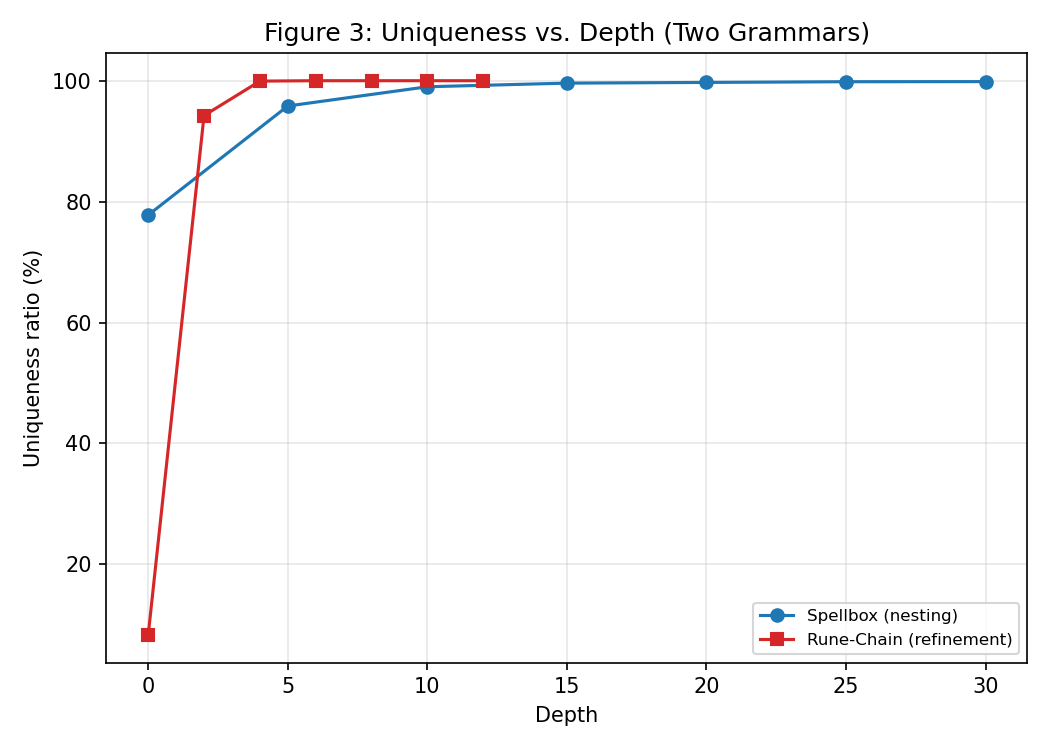
\includegraphics[keepaspectratio,alt={Figure 3: Uniqueness vs. depth, Spellbox vs. Rune-Chain}]{figures/figure3_uniqueness_two_grammars.png}}

\textbf{Figure 3.} Uniqueness ratio vs. depth for
Spellbox\textquotesingle s nesting operator and
Rune-Chain\textquotesingle s refinement operator. Rune-Chain saturates
to near-100\% uniqueness by depth 4, faster than
Spellbox\textquotesingle s more gradual approach to the same ceiling;
both grammars converge to a maximally-unique regime at high depth, but
at different rates, consistent with Rune-Chain\textquotesingle s smaller
flat-baseline solution space (8\% uniqueness at depth 0 vs.
Spellbox\textquotesingle s 78\%).

\pandocbounded{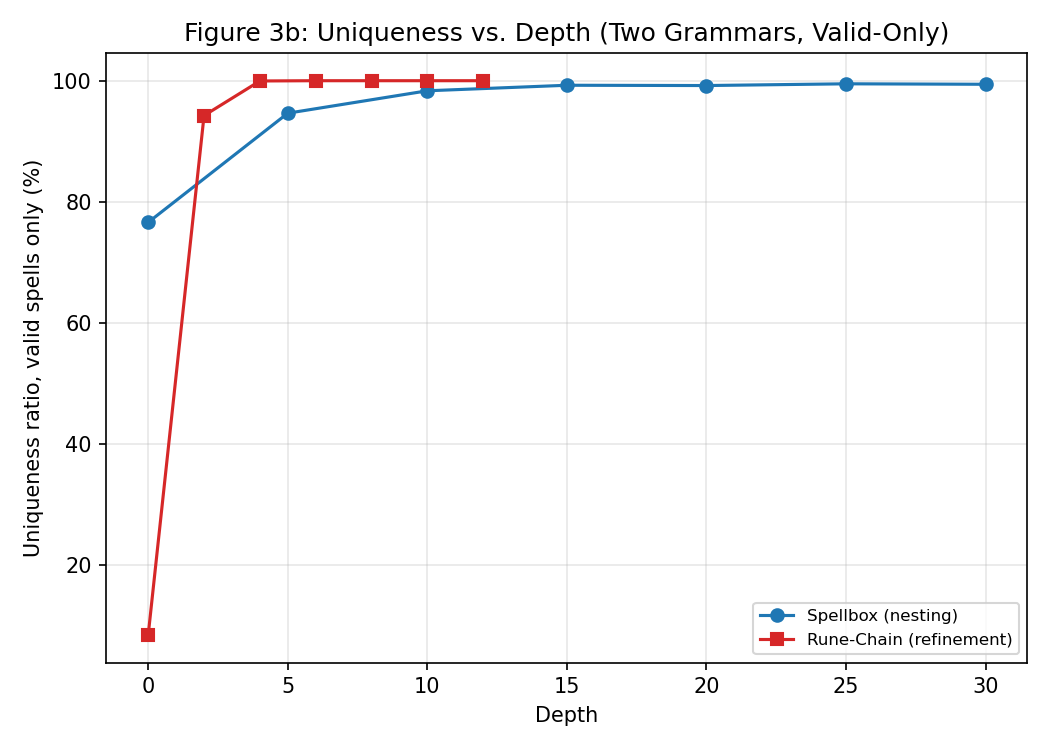
\includegraphics[keepaspectratio,alt={Figure 3b: Uniqueness vs. depth, valid-only}]{figures/figure3b_uniqueness_two_grammars_valid_only.png}}

\textbf{Figure 3b.} The same comparison recomputed under the
validity-gated uniqueness metric (Section 2.2). The two curves are
visually indistinguishable from Figure 3: chaining\textquotesingle s
validity is pinned near 100\% by design (see below), so its valid-only
curve is identical to its all-spells curve, and
refinement\textquotesingle s curve shifts by less than a point at any
depth. This is the expected outcome, not a null result: it is a clean
internal-consistency check that the validity-gating fix behaves
correctly and introduces no spurious change where none is expected.

\textbf{Valid-only recheck.} Applying the validity-gated metrics from
Section 2.2 to Rune-Chain gives an internal-consistency check that was
expected in advance: chaining\textquotesingle s validity is pinned at
essentially 100\% across all tested depths, because chain-adjacency
violations in this grammar are implemented as warnings rather than hard
validity errors (Section 3.6). Accordingly, chaining\textquotesingle s
valid-only uniqueness and discovery-rate numbers are \textbf{identical
to its all-spells numbers} to within noise (e.g., discovery rate at
chaining = 4, run 30: 69.5\% both all-spells and valid-only).
Refinement, which does carry real validity loss (89.5\% at depth 0 down
to 52.6\% at depth 12), shows the same pattern already established for
Spellbox: negligible movement between the all-spells and valid-only
figures (uniqueness at refinement = 0: 8.3\% all-spells vs. 8.4\%
valid-only; at refinement = 4: 99.9\% vs. 100.0\%), because
refinement\textquotesingle s validity stays fairly high across the
tested range. This is reassuring evidence that the validity-gating fix
is implemented correctly, since it produces exactly the "no effect where
none is expected" result the chaining operator\textquotesingle s design
predicts, rather than an arbitrary shift attributable to some other
change.

\subsubsection{3.8 Generality Check: A Constraint-Aware
Generator}\label{38-generality-check-a-constraint-aware-generator}

To determine whether validity loss under depth (Section 3.2) is an
intrinsic cost of compositional structure or an artifact of one
specific, fixable design decision, we built a constraint-aware generator
variant that changes exactly one thing: when constructing a Radial
composition symbol
(\texttt{\{\ composition:\ "Radial",\ sigils:\ {[}a,\ b{]}\ \}}), the
second sigil is sampled only from sigils compatible with the first (per
the existing \texttt{compatibility.ts} table), falling back to
uniform-random choice only for \texttt{Light}, which has no compatible
partner. Everything else (sign counts, nesting/linking recursion,
reversed-sign probability, symbol-option selection) is unchanged.

\begin{table*}[t]
\centering
\begin{tabular}{@{}cccc@{}}
\toprule
Depth & Baseline Validity \% & Constraint-Aware Validity \% & Absolute
Gain \\
\midrule
0 & 87.90 & 93.63 & +5.7 pts \\
10 & 56.00 & 71.95 & +15.95 pts \\
20 & 36.10 & 55.02 & +18.9 pts \\
30 & 25.70 & 43.38 & +17.7 pts \\
\bottomrule
\end{tabular}
\end{table*}

The absolute validity gain grows with depth (more Radial-composition
draws per spell means more opportunities for the one-line fix to
matter), recovering \textbf{17.7-18.9 percentage points of validity at
high depth} from a single, narrowly-targeted change. Critically,
\textbf{uniqueness ratio and discovery rate are essentially unchanged}
between generators (e.g., at nesting depth 20: uniqueness 0.997 baseline
vs. 0.996 constraint-aware; final discovery rate 95.65\% vs. 95.60\%,
well under a 1-point difference). This confirms composition-symbol
incompatibility, not the nesting/linking structure itself, is the
dominant driver of Spellbox\textquotesingle s validity loss under depth:
biasing one random decision toward known-compatible outcomes recovers a
large fraction of otherwise-invalid spells without touching the size or
novelty dynamics of the reachable spell space at all.

\textbf{Valid-only recheck reveals a new finding invisible to the
original metric.} Applying the validity-gated discovery-rate metric
(Section 2.2) to this same generator comparison shows that "essentially
unchanged" is true under the all-spells metric but not under valid-only:
at nesting depth 20, constraint-aware\textquotesingle s valid-only
discovery rate (92.27\%) pulls measurably ahead of
baseline\textquotesingle s (89.16\%), a \textbf{3.1-point gap} that the
original all-spells comparison (95.60\% vs. 95.65\%, under 1 point
apart) could not detect. The same pattern holds at depth 10 (85.59\%
constraint-aware vs. 82.94\% baseline, valid-only) though it is smaller
in absolute terms. The mechanism is straightforward: constraint-aware
has fewer invalid spells "crowding out" the valid-only denominator, so a
larger share of its valid spells are newly-seen valid signatures in each
batch. We report this as a genuinely new, secondary finding rather than
a correction to the existing claim: the constraint-aware
fix\textquotesingle s primary, already-reported benefit is its direct
validity gain (Section 3.8\textquotesingle s main table), but it also
produces a modest, previously-undetectable improvement in valid-only
discovery rate at high depth, on top of that validity gain. Uniqueness
ratio itself remains essentially unchanged between generators under
valid-only as well (Section 2 of the data underlying this section: e.g.,
0.9920 baseline vs. 0.9933 constraint-aware at depth 20), so this new
finding is specific to discovery rate, not a broader reassessment of the
generator comparison.

\pandocbounded{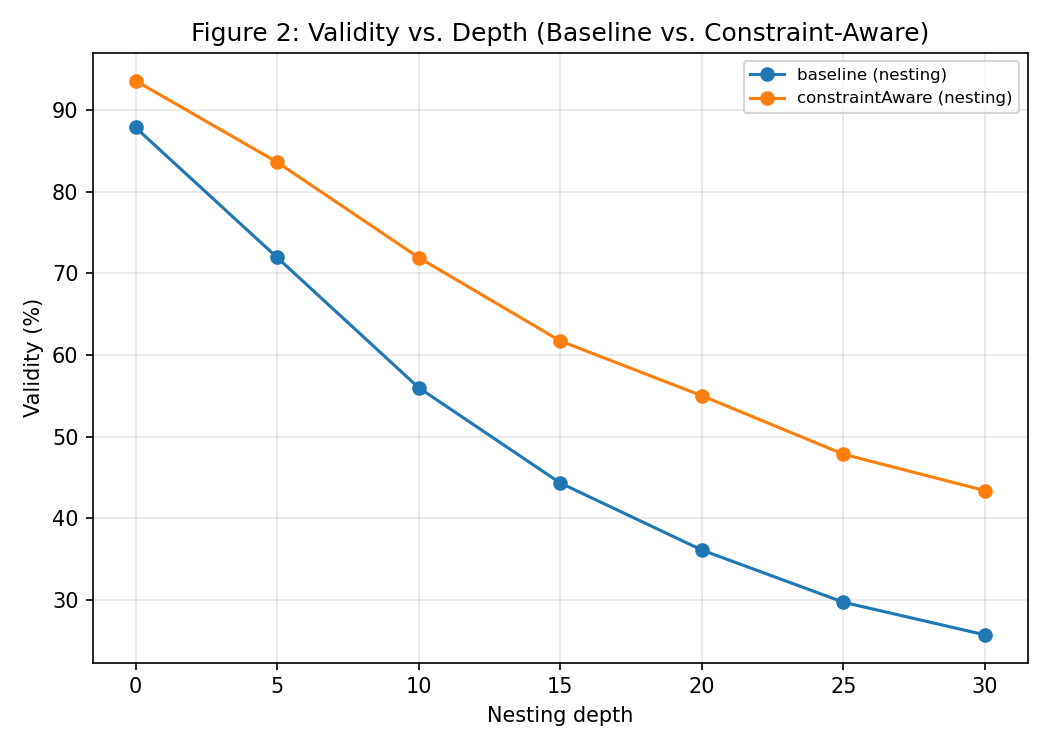
\includegraphics[keepaspectratio,alt={Figure 2: Validity vs. depth, baseline vs. constraint-aware}]{figures/figure2_validity_baseline_vs_constraint_aware.png}}

\textbf{Figure 2.} Validity (\%) vs. nesting depth for the baseline
generator and the constraint-aware variant. The constraint-aware curve
sits consistently above baseline at every depth, with the absolute gap
widening from +5.7 points at depth 0 to +18.9 points at depth 20, before
narrowing slightly to +17.7 points at depth 30.

\subsubsection{3.9 Runtime Analysis: Generation Time vs.
Depth}\label{39-runtime-analysis-generation-time-vs-depth}

We instrumented \texttt{generateBulkMetrics()} to measure wall-clock
generation time (5 repeated timing samples per depth, 1200 spells per
sample) across the same depth range used in Section 3.2, for both
operators:

\begin{table*}[t]
\centering
\begin{tabular}{@{}ccc@{}}
\toprule
Depth & Nesting: mean time (ms) & Linking: mean time (ms) \\
\midrule
0 & 6.6 ± 0.8 & N/A \\
5 & 14.4 ± 0.3 & 14.9 ± 1.5 \\
10 & 24.4 ± 0.8 & 24.7 ± 0.6 \\
15 & 35.1 ± 2.9 & 34.3 ± 2.3 \\
20 & 42.7 ± 1.1 & 43.5 ± 0.8 \\
25 & 52.3 ± 3.0 & 51.3 ± 1.9 \\
30 & 59.4 ± 1.1 & 58.4 ± 1.0 \\
\bottomrule
\end{tabular}
\end{table*}

\pandocbounded{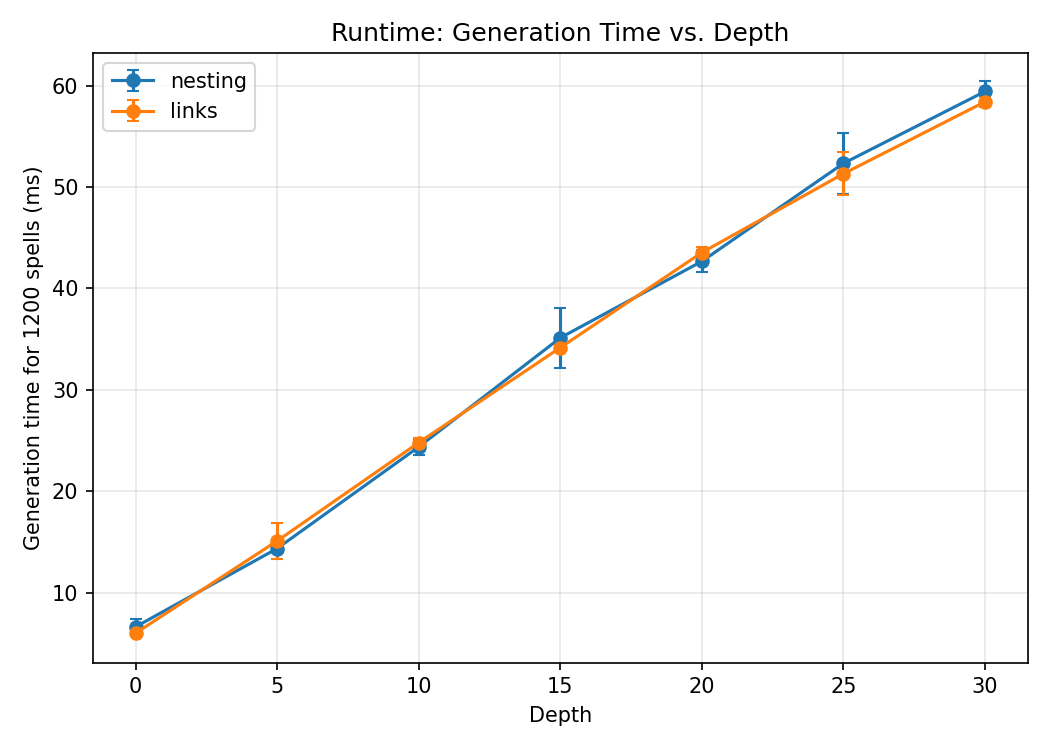
\includegraphics[keepaspectratio,alt={Figure: Runtime vs. depth}]{figures/figure_runtime_vs_depth.png}}

Generation time grows approximately linearly with depth for both
operators (roughly 1.8 ms per depth level beyond a small fixed overhead
at depth 0), and the two operators track each other closely at every
depth (within 1-2 ms), consistent with both recursing the same number of
times per spell (one call per nesting level or per link) with comparable
per-call cost. At the depths and amounts used throughout this paper (≤
1200 spells, ≤ depth 30), total generation time remains under 60 ms, so
runtime is not a practical constraint on any experiment reported here;
it would become relevant only at substantially larger amounts or depths
than tested in this study.

\subsubsection{3.10 Nominal vs. Effective Search-Space Size: Quantifying
Sampler
Bias}\label{310-nominal-vs-effective-search-space-size-quantifying-sampler-bias}

\textbf{Motivation.} A first pass at this question (computing a
combinatorial upper bound on the number of distinct spell signatures
reachable at a given nesting depth) suggested the theoretical space
grows so explosively with depth that it is effectively unlimited for any
realistic sampling budget, a conclusion that, if taken at face value,
makes this section\textquotesingle s finding a nearly arithmetic
consequence of exponentiation rather than a substantive empirical
result. That combinatorial bound is still useful as a \emph{nominal}
space size, but treating it as the relevant measure of "how large is the
space this experiment actually explores" turns out to be the wrong
question. This section instead asks: given the discovery-rate data
already collected (Section 3.3), how large is the space the sampler is
\emph{behaviorally} exploring, and how does that compare to the nominal
combinatorial bound? The gap between the two, and its mechanism, is the
actual result.

\textbf{Nominal space size.} Per generation node, the grammar draws: a
\textbf{central symbol} (5 sigils + 5 transformations + 15 unordered
sigil-pair classes = 25 equivalence classes), and a \textbf{sign set}
(one of 3 signOption branches, each drawing 1-3 signs from independent
5-element categories with a binary reversed flag per sign; option 1: 5×2
= 10; option 2: (5×2)×(5×2 + 5×2) = 200; option 3: (5×2)×(5×2)×(5×2) =
1,000; total 1,210 sign-set classes). This gives \textbf{30,250
equivalence classes per node}, matching the exact equivalence relation
used by \texttt{signature()} (which sorts symbol/sign multisets, so
order within a node does not distinguish signatures). Compounding
multiplicatively across nesting depth, since each additional level
chains another independent node\textquotesingle s choices into the same
signature, gives the nominal upper bound \texttt{30,250\^{}(depth+1)}
reported in the "Nominal space" column below.

\textbf{Effective space size, via occupancy inversion.} The
discovery-rate sweep (Section 3.3) re-rolls the same generation shape 30
times per seed, tracking how many of each batch\textquotesingle s 1200
spells are structurally new versus a repeat of a previously-seen
signature. If a sampler draws uniformly from an effective space of size
\texttt{N\_eff}, the probability that a fresh draw collides with any of
the \texttt{k} previously-seen signatures is approximately
\texttt{k\ /\ N\_eff} (an occupancy/birthday-problem approximation,
valid while \texttt{k\ ≪\ N\_eff}). We already have, for every run in
every seed, both the observed repeat probability
(\texttt{repeats\ /\ total} for that batch) and the exact cumulative
count of previously-seen signatures \texttt{k} going into that batch
(\texttt{cumulativeUnique\ −\ newCount} from the prior run). Inverting
the approximation gives a direct, per-run estimate of the
sampler\textquotesingle s effective space size:
\texttt{N\_eff\ =\ k\ /\ observed\_repeat\_probability}. We compute this
at each of the last 10 runs of each seed\textquotesingle s 30-run
sequence (where \texttt{k} is largest and the estimate is most stable)
and average across seeds and runs:

\begin{table*}[t]
\centering
\begin{tabular}{@{}cccc@{}}
\toprule
Depth & Nominal space (combinatorial upper bound) & Effective space
(mean ± std, occupancy-inverted) & Gap (orders of magnitude) \\
\midrule
0 & 3.03 × 10⁴ & (1.06 ± 0.04) × 10⁴ & 0.5 \\
5 & 7.66 × 10²⁶ & (1.08 ± 0.10) × 10⁵ & 21.9 \\
10 & 1.94 × 10⁵² & (2.63 ± 0.34) × 10⁵ & 43.9 \\
20 & 1.25 × 10¹⁰³ & (6.84 ± 1.10) × 10⁵ & 88.3 \\
\bottomrule
\end{tabular}
\end{table*}

At depth 0, nominal and effective space size agree to within a factor of
\textasciitilde3 (0.5 orders of magnitude), exactly what
uniform-sampling behavior over the full nominal space should look like,
and a sanity check that the occupancy-inversion method itself is sound
(the residual factor is consistent with the nominal figure being an
upper bound before accounting for further signature collapsing at the
sign-multiset level). The moment nesting is introduced, the two measures
diverge catastrophically: by depth 20, the nominal space has grown to
1.25 × 10¹⁰³ while the effective space the sampler actually behaves as
if it is drawing from has grown only to \textasciitilde6.8 × 10⁵, a
\textbf{gap of 88 orders of magnitude}, and the gap widens (not
stabilizes) as depth increases across the tested range.

\textbf{Valid-only recheck.} Restricting the same occupancy-inversion
procedure to valid spells only (Section 2.2) gives:

\begin{table*}[t]
\centering
\begin{tabular}{@{}cccccc@{}}
\toprule
Depth & Nominal space & Effective space (all-spells, mean) & Effective
space (valid-only, mean) & Gap, all (orders of mag.) & Gap, valid-only
(orders of mag.) \\
\midrule
0 & 3.03 × 10⁴ & 1.06 × 10⁴ & 0.877 × 10⁴ & 0.5 & 0.5 \\
5 & 7.66 × 10²⁶ & 1.08 × 10⁵ & 0.602 × 10⁵ & 21.9 & 22.1 \\
10 & 1.94 × 10⁵² & 2.63 × 10⁵ & 0.870 × 10⁵ & 43.9 & 44.3 \\
20 & 1.25 × 10¹⁰³ & 6.84 × 10⁵ & 0.966 × 10⁵ & 88.3 & 89.1 \\
\bottomrule
\end{tabular}
\end{table*}

The headline, log-scale "gap in orders of magnitude" is barely affected
by the correction (88.3 → 89.1 at depth 20), since it is a measure
against an astronomically large nominal space and a factor-of-7 change
in the effective-space estimate barely registers on a log scale spanning
100+ orders of magnitude. But the \emph{absolute} effective-space
estimate at depth 20 shrinks substantially once restricted to valid
spells: from 6.84 × 10⁵ to 0.966 × 10⁵, a factor of \textasciitilde7
(684K → 96.6K). We read this as \textbf{strengthening, not weakening},
this section\textquotesingle s argument: the true effective space the
sampler explores, once restricted to spells that are actually valid, is
even smaller than the original (all-spells) figure reported, reinforcing
the claim that the sampler behaviorally explores a far smaller space
than the nominal combinatorial bound suggests.

\textbf{Mechanism: sampler bias from the depth-is-a-ceiling design.}
This gap is explained by the same mechanism identified in Section
3.2\textquotesingle s achieved-depth analysis: each spell independently
draws its own nesting depth uniformly on \texttt{{[}0,\ ceiling{]}}
rather than every spell reaching the ceiling, so a "depth = 20"
run\textquotesingle s actual sample is dominated by shallow spells (mean
achieved depth 9.81, not 20). The nominal-space calculation assumes
every node in its count exists \emph{at} the stated depth; the sampler,
in reality, spends most of its draws at much shallower depths where the
per-node combinatorics have had far fewer compounding rounds to explode.
Because the nominal space is a product of per-node class counts raised
to the node-count power, and the achieved node count is concentrated
near half the ceiling rather than at the ceiling itself, an enormous
share of the nominal space\textquotesingle s volume (everything
reachable only by spells that actually draw depths in the upper half of
\texttt{{[}0,\ ceiling{]}}) is sampled so rarely across a 30-run,
1200-spell-per-run budget that it contributes negligibly to the observed
collision rate. The effective space size measured here is therefore not
"the size of the space Spellbox\textquotesingle s grammar can produce"
but "the size of the space this specific per-spell-uniform sampling
strategy behaves as though it is drawing from," a distinction the
nominal-space number alone cannot make visible.

\textbf{Reframing the result.} The contribution of this section is not
"the theoretical space is astronomically large" (Section 3.2 and the
mechanism above already establish that the depth ceiling
doesn\textquotesingle t force deep sampling, making combinatorial
explosion an expected and near-arithmetic consequence). The contribution
is a \textbf{general, reusable method for quantifying the gap between a
compositional generator\textquotesingle s nominal combinatorial capacity
and the effective capacity a given sampling strategy actually
exercises}: (1) derive the nominal space size from the
grammar\textquotesingle s equivalence-class structure, (2) use observed
repeat/collision rates plus cumulative unique-signature counts to invert
an effective space size via the occupancy approximation, and (3)
attribute the gap to a specific, identifiable property of the sampling
strategy (here, independent per-spell uniform depth draws against a
fixed ceiling) rather than treating "large nominal space" and "high
discovery rate" as if they were the same finding. Any PCG system with a
compositional grammar and a non-exhaustive sampling strategy admits the
same two measurements and the same gap-attribution exercise; a grammar
whose sampler \emph{does} force every generated item to the nominal
depth would be expected to show a much smaller nominal-vs-effective gap,
which would itself be a useful diagnostic for comparing sampler designs
across generators (cf. Withington and Tokarchuk\textquotesingle s and
Barthet et al.\textquotesingle s generative-space comparison methods,
Section 1.2).

This also sharpens the interpretation of Section 3.3\textquotesingle s
discovery-rate results: a high, slowly-decaying discovery rate at
nominal depth 20 is not evidence that generation is exploring a
near-limitless space (the nominal-space framing), nor is it merely "the
space is so large no budget could exhaust it"; it is evidence that the
sampler is effectively drawing from a space of a few hundred thousand
signatures (not 10¹⁰³), which a 36,000-spell cumulative budget (30 runs
× 1200) is still far from saturating, but which is a concrete,
measurable, and much smaller quantity than the grammar\textquotesingle s
raw combinatorial capacity would suggest.

\subsubsection{3.11 Complexity
Distribution}\label{311-complexity-distribution}

To check whether compositional depth widens the distribution of spell
complexity (raw score) or merely shifts its mean, we sampled 1200 spells
at depths 0, 10, and 30 for both operators and plotted the raw-score
density:

\pandocbounded{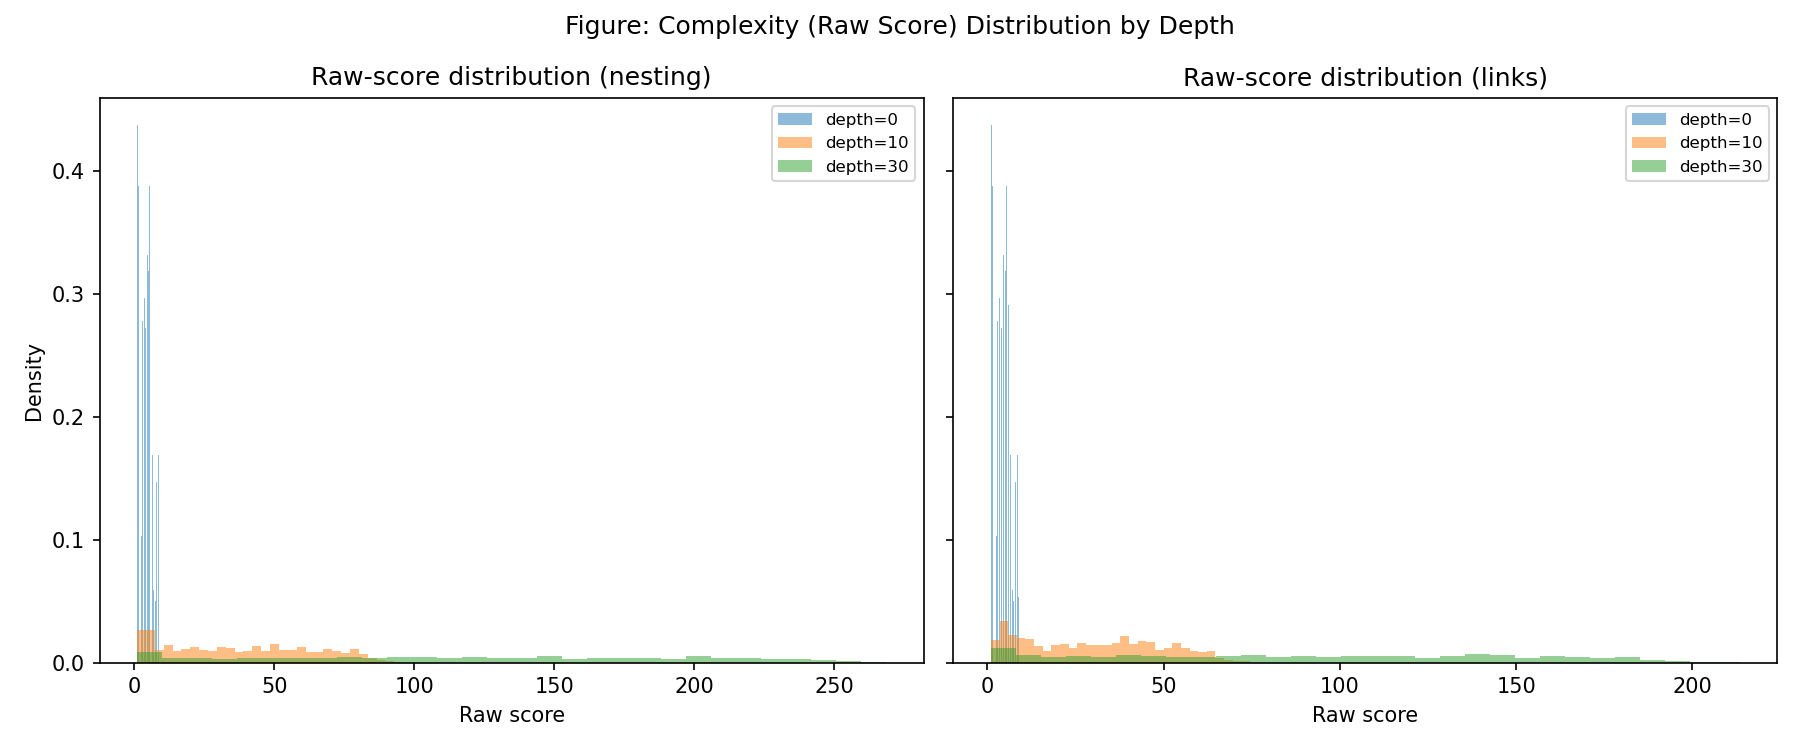
\includegraphics[keepaspectratio,alt={Figure: Complexity distribution by depth}]{figures/figure_complexity_histograms.png}}

\begin{table*}[t]
\centering
\begin{tabular}{@{}ccccc@{}}
\toprule
Depth & Nesting: mean ± std & Nesting: range & Linking: mean ± std &
Linking: range \\
\midrule
0 & 4.16 ± 3.0 & {[}0, \textasciitilde18{]} & 4.16 ± 3.0 & {[}0,
\textasciitilde18{]} \\
10 & 38.1 ± 24.8 & {[}0, \textasciitilde150{]} & 29.5 ± 17.6 & {[}0,
\textasciitilde110{]} \\
30 & 120.0 ± 55.4 & {[}0, \textasciitilde280{]} & 91.5 ± 43.5 & {[}0,
\textasciitilde215{]} \\
\bottomrule
\end{tabular}
\end{table*}

The distribution does not simply translate rightward with depth: its
\textbf{spread grows much faster than a pure shift would produce}:
standard deviation rises from 3.0 at depth 0 to 55.4 at depth 30 for
nesting (an 18.5× increase, compared to a 28.4× increase in the mean
itself), and the histogram shows the depth-30 distribution is nearly
flat/uniform across a wide range rather than a narrow bump displaced
from the depth-0 peak. This confirms compositionality\textquotesingle s
effect on complexity is not just "spells get bigger on average" but
"spells become far more heterogeneous in size": at high depth, the
amount of compounding a given spell happens to receive (via its
independently-drawn nesting/linking count per spell, Section 2.1)
dominates its final complexity far more than at shallow depth, where
nearly every spell is close to the same small size.

\subsection{4. Discussion}\label{4-discussion}

\subsubsection{4.1 H1 and H2 Together}\label{41-h1-and-h2-together}

H1 and H2 describe a specific tradeoff space rather than two unrelated
effects: the same compositional operators that sustain a high discovery
rate (H1) are, in Spellbox, the ones spending validity to do so (H2).
Section 3.2\textquotesingle s geometric-decay baseline shows that H2, as
originally stated ("depth trades validity for complexity"), is close to
a definitional consequence of two more basic facts: validity is a
conjunction of independent per-node checks, and each additional unit of
nominal depth adds nodes that are individually error-prone at a fixed,
measured rate: a null model that predicts most of the observed decay
shape once the achieved (not nominal) node count is used. The part of H2
that is \emph{not} a near-arithmetic consequence of those two facts, and
is therefore the genuinely interesting result, is Section
3.8\textquotesingle s finding: a substantial share of the per-node error
rate itself is attributable to one specific, correctable random-choice
bottleneck (composition-symbol sigil pairing), not an intrinsic property
of composition, and fixing it recovers up to \textasciitilde19 points of
validity at high depth while leaving discovery-rate dynamics completely
untouched. This reframes H2\textquotesingle s practical implication:
depth\textquotesingle s validity cost in this grammar is partly a
\emph{tunable generator-design} cost, not an unavoidable structural one.
The second-grammar check (Section 3.7) reinforces this from a different
angle: its linking-equivalent operator paid no validity cost at all,
because its author (by design choice, not oversight) made
chain-adjacency violations a warning rather than an error. Taken
together, whether a compositional operator "costs" validity in a given
grammar depends on how tightly that grammar\textquotesingle s validity
rules are coupled to that operator\textquotesingle s structural growth,
not on compositional depth in the abstract.

\subsubsection{4.2 Confound: Normalization Function
Choice}\label{42-confound-normalization-function-choice}

Because the tier boundaries were originally calibrated against
Exponential normalization, the same underlying raw score produces
different tier labels depending on which normalization function is
applied (e.g., at depth 10 in the original single-seed sweep: Master
under Sigmoid, Adept under Exponential, Apprentice under Arctan, for
numerically identical spells). This is a labeling artifact, not a
generation-behavior difference, and all cross-row complexity comparisons
in this paper are made only within a fixed normalization function
(Exponential, for all multi-seed experiments) for that reason.

\subsubsection{4.3 Threats to Validity}\label{43-threats-to-validity}

\textbf{Internal Validity.} The core risk to internal validity is that
observed effects are artifacts of the random generation process itself
rather than genuine consequences of nesting/linking structure. We
mitigate this in three ways: (1) every depth-sweep and discovery-rate
result is reported as a mean ± standard deviation across 5 independent
seeds (Sections 3.2, 3.3), with the confidence intervals and
Cohen\textquotesingle s d effect sizes in Section 3.4 confirming the
flat-vs-nesting and flat-vs-linking validity gaps are far outside what
seed noise could produce (non-overlapping 95\% CIs and
\textbar d\textbar{} \textgreater{} 14 at every tested depth); (2) the
nominal-vs-effective space-size analysis (Section 3.10) shows the
observed discovery-rate trends reflect a specific, measured effective
space size rather than being taken on faith from the nominal
combinatorial bound; (3) we now directly report that each generated
spell independently draws its own nesting depth or link count up to the
run\textquotesingle s ceiling (Section 2.1, quantified in Section
3.2\textquotesingle s achieved-depth table) rather than every spell
being forced to the maximum; this is no longer an unquantified threat,
since Section 3.2 reports the full achieved-depth distribution at each
ceiling and Section 3.10 traces the nominal-vs-effective space gap
directly to this mechanism, but it remains a design property of the
generator we did not alter for this study (Section 3.5), so "depth = 20"
should still be read throughout as a ceiling on a distribution, not a
level every spell reaches.

\textbf{A fourth internal-validity threat, identified and corrected
during this study: validity/uniqueness conflation.} We found, during
this study, that the original uniqueness-ratio and discovery-rate
tracking counted a spell\textquotesingle s \texttt{signature()} as
"unique" or "newly discovered" without gating on that
spell\textquotesingle s validity (Section 2.2). This is an
internal-validity threat because it means a metric intended to measure
novelty of \emph{sound} generator output could instead be partly
measuring novelty of malformed output, which is a different (and less
interesting) quantity. We quantified the magnitude of this threat
directly rather than assuming it away: for uniqueness ratio, the effect
is small, at most \textasciitilde1.2 percentage points of difference at
any tested depth (Section 3.2); for discovery rate, the effect is larger
and grows with depth, reaching 6-7 percentage points by run 30 at
nesting/linking depth 20 (Section 3.3), and it is large enough to
require restating the abstract\textquotesingle s headline gap figure
(from 64-83 points to roughly 60-78 points, valid-only). We corrected
the underlying tracking code to add a parallel, validity-gated metric
alongside every original one (rather than silently replacing the
original), and we report both throughout this paper so a reader can
judge the magnitude of the correction directly rather than trust a
single recomputed number. Both of this paper\textquotesingle s
hypotheses (H1, H2) hold under the corrected metric (Section 3.6); this
threat was real and is now quantified and disclosed, but it does not
overturn either of the paper\textquotesingle s core conclusions.

\textbf{External Validity.} All quantitative findings are demonstrated
on two grammars only (Spellbox and the purpose-built Rune-Chain second
grammar, Section 3.7), both toy, synthetic domains with small
(5-primitive) vocabularies and simple pairwise validity rules.
Rune-Chain was built by the same research process being evaluated, which
is a weaker generality test than an independently-designed, pre-existing
grammar would provide (though its H2 divergence for the chaining
operator, Section 3.6, is informative precisely because it was not tuned
to agree with Spellbox\textquotesingle s results). Neither grammar
resembles a production-scale PCG system (e.g., full game-content
generators with hundreds of primitives and cross-cutting constraints),
so claims here should be read as "this pattern is not unique to one
specific rule set" rather than "this pattern holds for compositional PCG
systems in general." The discovery-rate experiments are also bounded to
a 30-re-roll window (Sections 3.3, 3.7); the logarithmic best-fit
implies discovery rate keeps declining slowly rather than plateauing
within that window, so whether the deepest compositional shapes ever
saturate outside this window is untested.

\textbf{Construct Validity.} This paper operationalizes "novelty
saturation" as \textbf{discovery rate}: the fraction of each re-rolled
batch that is structurally new by the \texttt{signature()} equivalence
relation (Section 2.2). This is a proxy, not a direct measurement of the
underlying concept: \texttt{signature()} collapses spells that differ
only in sign order or in un-tracked structural details into the same
class, so discovery rate measures saturation of the \emph{signature
space}, which may be coarser or finer than what a human player would
perceive as "a new spell." Section 3.10\textquotesingle s
effective-space-size estimate reinforces this concern from a different
angle: a persistently high discovery rate is consistent both with "the
grammar is genuinely rich" and with "the signature equivalence relation
is simply too coarse to ever register a collision at the effective space
sizes measured there (on the order of 10⁴-10⁶ signatures)"; this paper
cannot fully distinguish those two explanations from discovery-rate data
alone, and doing so would require an independent human-judgment baseline
(e.g., sampling spell pairs the signature relation calls distinct and
asking human raters whether they are meaningfully different) that is out
of scope for this study. Because we cannot rule out the
coarser-signature-relation explanation, every discovery-rate and novelty
claim in this paper should be read as scoped to \emph{novelty under
\texttt{signature()}}, not validated against human-perceived novelty; we
state this in the abstract as well as here, rather than only here, so
the paper\textquotesingle s scope is not overstated by readers who skip
Section 4.3. Similarly, \textbf{validity} is a binary construct
(structurally sound vs. not, per the validator\textquotesingle s
error-level checks; Section 2.2) that treats all validity violations as
equivalent, when in practice a single incompatible composition-symbol
pair might be a materially different failure than a missing Control
sign; Section 3.8\textquotesingle s constraint-aware intervention shows
these are not evenly distributed, so "validity \%" is a coarser signal
than the underlying failure modes it aggregates.

Two further threats apply across all three categories: nesting and
linking are compared at matched \emph{depth} values, not matched
\emph{raw-score} values (Section 3.2), so a depth-matched comparison is
not a complexity-matched one; and the constraint-aware generator
(Section 3.8) targets exactly one identified validity-loss mechanism,
leaving smaller sources of invalidity unaddressed and still contributing
to the residual validity gap at high depth.

\subsection{5. Conclusion}\label{5-conclusion}

This study asked how compositional operators affect novelty saturation
in a constrained procedural spell grammar, and tested it with several
converging lines of evidence: single-seed sweeps, 5-seed multi-seed
sweeps with variance reporting, per-seed AIC/BIC-based curve fitting, an
independent generator-design intervention, a fully independent second
grammar, and a nominal-vs-effective search-space analysis. H1
(compositional operators delay saturation) is well-supported and
replicates cleanly in an independent grammar. H2 (depth trades validity
for complexity) holds cleanly in Spellbox for both operators, and in the
second grammar for its nesting-equivalent operator, but a validity cost
is not automatic for a linking-equivalent operator: it depends on
whether that grammar\textquotesingle s rules are actually sensitive to
what linking changes structurally. A geometric-decay baseline (Section
3.2) shows most of H2\textquotesingle s shape is close to a definitional
consequence of two more basic facts (validity as a conjunction of
independent per-node checks, and depth as a per-spell ceiling rather
than a level), which sharpens rather than weakens the
paper\textquotesingle s most interesting validity finding: a follow-up
experiment isolating exactly one validity-loss mechanism
(composition-symbol pairing) showed a large fraction of
Spellbox\textquotesingle s \emph{residual}, non-definitional validity
cost is a fixable generator-design choice, not an unavoidable tax on
compositional depth itself. Separately, this paper\textquotesingle s
search-space analysis (Section 3.10) contributes a general, reusable
method (nominal combinatorial space size versus occupancy-inverted
effective space size from observed collision rates) for quantifying how
much of a compositional generator\textquotesingle s raw capacity a given
sampling strategy actually reaches; applied here, it shows
Spellbox\textquotesingle s per-spell-uniform depth sampling reaches an
effective space many orders of magnitude smaller than its nominal
combinatorial capacity, and traces that gap to the same
depth-is-a-ceiling mechanism underlying the H2 reframing above. Taken
together, the expressiveness-versus-soundness tradeoff observed here is
real, but partially negotiable by grammar and sampler design rather than
fixed by the choice to use composition operators at all. During this
study we also found, quantified, and corrected a methodological bug in
which the uniqueness-ratio and discovery-rate metrics did not gate on
spell validity (Section 2.2); we consider the discovery and correction
of this bug, and the transparent reporting of both the original and
corrected figures throughout (Sections 3.2, 3.3, 3.5, 3.7, 3.8, 3.10,
4.3), part of this study\textquotesingle s rigor rather than a mark
against it, since the correction was caught before publication, its
magnitude was quantified precisely, and it was shown not to overturn
either H1 or H2 (Section 3.6). All findings remain scoped to novelty and
search-space size as measured under the \texttt{signature()} equivalence
relation; independently validating that relation against human judgments
of "meaningfully different" spells, extending discovery-rate sequences
well beyond 30 re-rolls, re-running the depth sweeps with a fixed
(rather than uniformly-drawn) per-spell depth, and testing additional
independently-designed grammars are the clearest directions for future
work.

\subsection{References}\label{references}

\textbf{Grammar-based / rule-based PCG}

\begin{itemize}
\tightlist
\item
  Stiny, G., and Gips, J. "Shape Grammars and the Generative
  Specification of Painting and Sculpture." \emph{IFIP Congress}, 1971.
\item
  Prusinkiewicz, P., and Lindenmayer, A. \emph{The Algorithmic Beauty of
  Plants}. Springer, 1990.
\item
  Müller, P., Wonka, P., Haegler, S., Ulmer, A., and Van Gool, L.
  "Procedural Modeling of Buildings." \emph{ACM SIGGRAPH}, 2006.
\item
  Dormans, J. "Adventures in Level Design: Generating Missions and
  Spaces for Action Adventure Games." \emph{Proceedings of the 2010
  Workshop on Procedural Content Generation in Games (PCGames)}, 2010.
\item
  Smith, A. M., and Mateas, M. "Variations Forever: Flexibly Generating
  Rulesets from a Sculptable Design Space of Mini-games." \emph{IEEE
  Conference on Computational Intelligence and Games (CIG)}, 2010.
\item
  Smith, A. M., and Mateas, M. "Answer Set Programming for Procedural
  Content Generation: A Design Space Approach." \emph{IEEE Transactions
  on Computational Intelligence and AI in Games (TCIAIG)}, 3(3), 2011.
\item
  Shaker, N., Togelius, J., and Nelson, M. J. \emph{Procedural Content
  Generation in Games: A Textbook and an Overview of Current Research}.
  Springer, 2016.
\end{itemize}

\textbf{Expressive range and generator evaluation}

\begin{itemize}
\tightlist
\item
  Smith, G., and Whitehead, J. "Analyzing the Expressive Range of a
  Level Generator." \emph{Proceedings of the 2010 Workshop on Procedural
  Content Generation in Games (PCGames)}, 2010.
\item
  Horn, B., Dahlskog, S., Shaker, N., Smith, G., and Togelius, J. "A
  Comparative Evaluation of Procedural Level Generators in the Mario AI
  Framework." \emph{Foundations of Digital Games (FDG)}, 2014.
\item
  Smith, G. "What Do We Value in Procedural Content Generation?"
  \emph{Foundations of Digital Games (FDG)}, 2017.
\item
  Summerville, A. "Expanding Expressive Range: Evaluation Methodologies
  for Procedural Content Generation." \emph{AIIDE}, 2018.
\item
  Cook, M., Colton, S., Gow, J., and Smith, G. "General Analytical
  Techniques for Parameter-Based Procedural Content Generators."
  \emph{IEEE Conference on Games (CoG)}, 2019.
\item
  Cook, M., Gow, J., Smith, G., and Colton, S. "Danesh: Interactive
  Tools for Understanding Procedural Content Generators." \emph{IEEE
  Transactions on Games}, 14(3), 2022, pp. 329-338.
\end{itemize}

\textbf{Diversity and novelty}

\begin{itemize}
\tightlist
\item
  Lehman, J., and Stanley, K. O. "Abandoning Objectives: Evolution
  Through the Search for Novelty Alone." \emph{Evolutionary
  Computation}, 19(2), 2011.
\item
  Togelius, J., Yannakakis, G. N., Stanley, K. O., and Browne, C.
  "Search-Based Procedural Content Generation: A Taxonomy and Survey."
  \emph{IEEE Transactions on Computational Intelligence and AI in Games
  (TCIAIG)}, 3(3), 2011.
\item
  Mouret, J.-B., and Clune, J. "Illuminating Search Spaces by Mapping
  Elites." \emph{arXiv:1504.04909}, 2015.
\item
  Pugh, J. K., Soros, L. B., and Stanley, K. O. "Quality Diversity: A
  New Frontier for Evolutionary Computation." \emph{Frontiers in
  Robotics and AI}, 3, 2016.
\item
  Gravina, D., Khalifa, A., Liapis, A., Togelius, J., and Yannakakis, G.
  N. "Procedural Content Generation through Quality Diversity."
  \emph{IEEE Conference on Games (CoG)}, 2019 (also
  \emph{arXiv:1907.04053}).
\end{itemize}

\textbf{Generative-space comparison}

\begin{itemize}
\tightlist
\item
  Withington, T., and Tokarchuk, L. "Compressing and Comparing the
  Generative Spaces of Procedural Content Generators."
  \emph{arXiv:2205.15133}.
\item
  Barthet, M., Liapis, A., and Yannakakis, G. N. "Generative Shift
  Analysis." \emph{arXiv:2309.05371}.
\end{itemize}

\textbf{Statistical methodology}

\begin{itemize}
\tightlist
\item
  Burnham, K. P., and Anderson, D. R. \emph{Model Selection and
  Multimodel Inference: A Practical Information-Theoretic Approach}. 2nd
  ed., Springer, 2002.
\end{itemize}

\textbf{Grammar-as-rule-system framing (background)}

\begin{itemize}
\tightlist
\item
  Martens, C. "Ceptre: A Language for Modeling Generative Interactive
  Systems." \emph{AIIDE}, 2015.
\item
  Smith, A. M., Nelson, M. J., and Mateas, M. "Ludocore: A Logical Game
  Engine for Modeling Videogames." \emph{IEEE Conference on
  Computational Intelligence and Games (CIG)}, 2010.
\end{itemize}

\textbf{If a future human-evaluation study is added (Section 4.3)}

\begin{itemize}
\tightlist
\item
  Cherry, E., and Latulipe, C. "Quantifying the Creativity Support
  Index." \emph{ACM Transactions on Computer-Human Interaction (TOCHI)},
  21(4), 2014.
\item
  Compton, K., and Mateas, M. "Casual Creators." \emph{International
  Conference on Computational Creativity (ICCC)}, 2015.
\end{itemize}

\end{document}
